\section{Point Cloud in Construction Sector}
For high quality mesh processing of hallway point cloud in Autodesk ReCap pro,it is needed to buy tokens so I decided to a explain a sample from Autodesk website.  A well known software for meshing the point cloud data related to building industry is Autodesk ReCap Pro. As an example I can select all or portion of point cloud data in ReCap Pro for further mesh processing \cite{ReCap}. \\

\noindent \textbf{First step}: Point Cloud Visualization in Autodesk ReCap pro
\begin{figure}[H]
  \centering
  \includegraphics[width= 0.9\textwidth]{Figures/Portion of Point Cloud.PNG}
  \caption[Picture of Visualized Point Cloud]{Picture of Visualized point cloud}
\end{figure}

\noindent \textbf{Second step}: Selection of all or portion of point cloud in Autodesk ReCap pro
\begin{figure}[H]
  \centering
  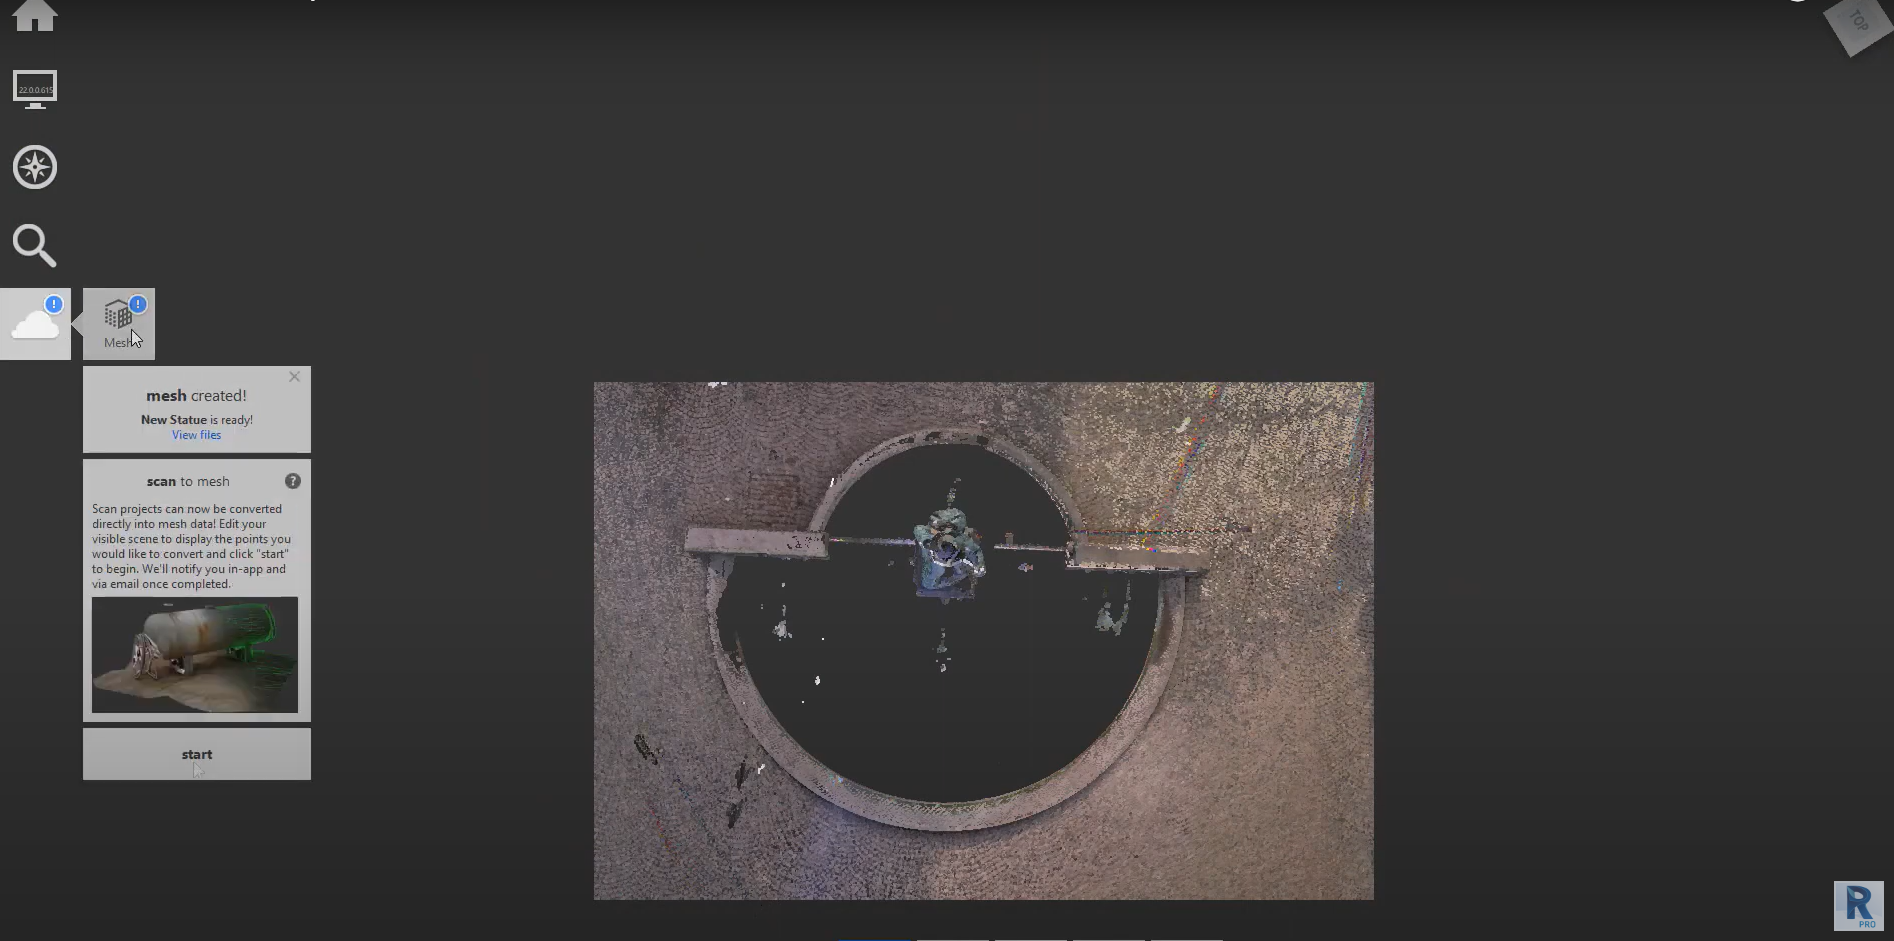
\includegraphics[width= 0.9\textwidth]{Figures/Mesh option.PNG}
  \caption[Portion of selectded Point Cloud]{Picture of selected portion of point cloud }
\end{figure}
\noindent \textbf{Final step}: Meshed point cloud in Autodesk ReCap pro
\begin{figure}[H]
  \centering
  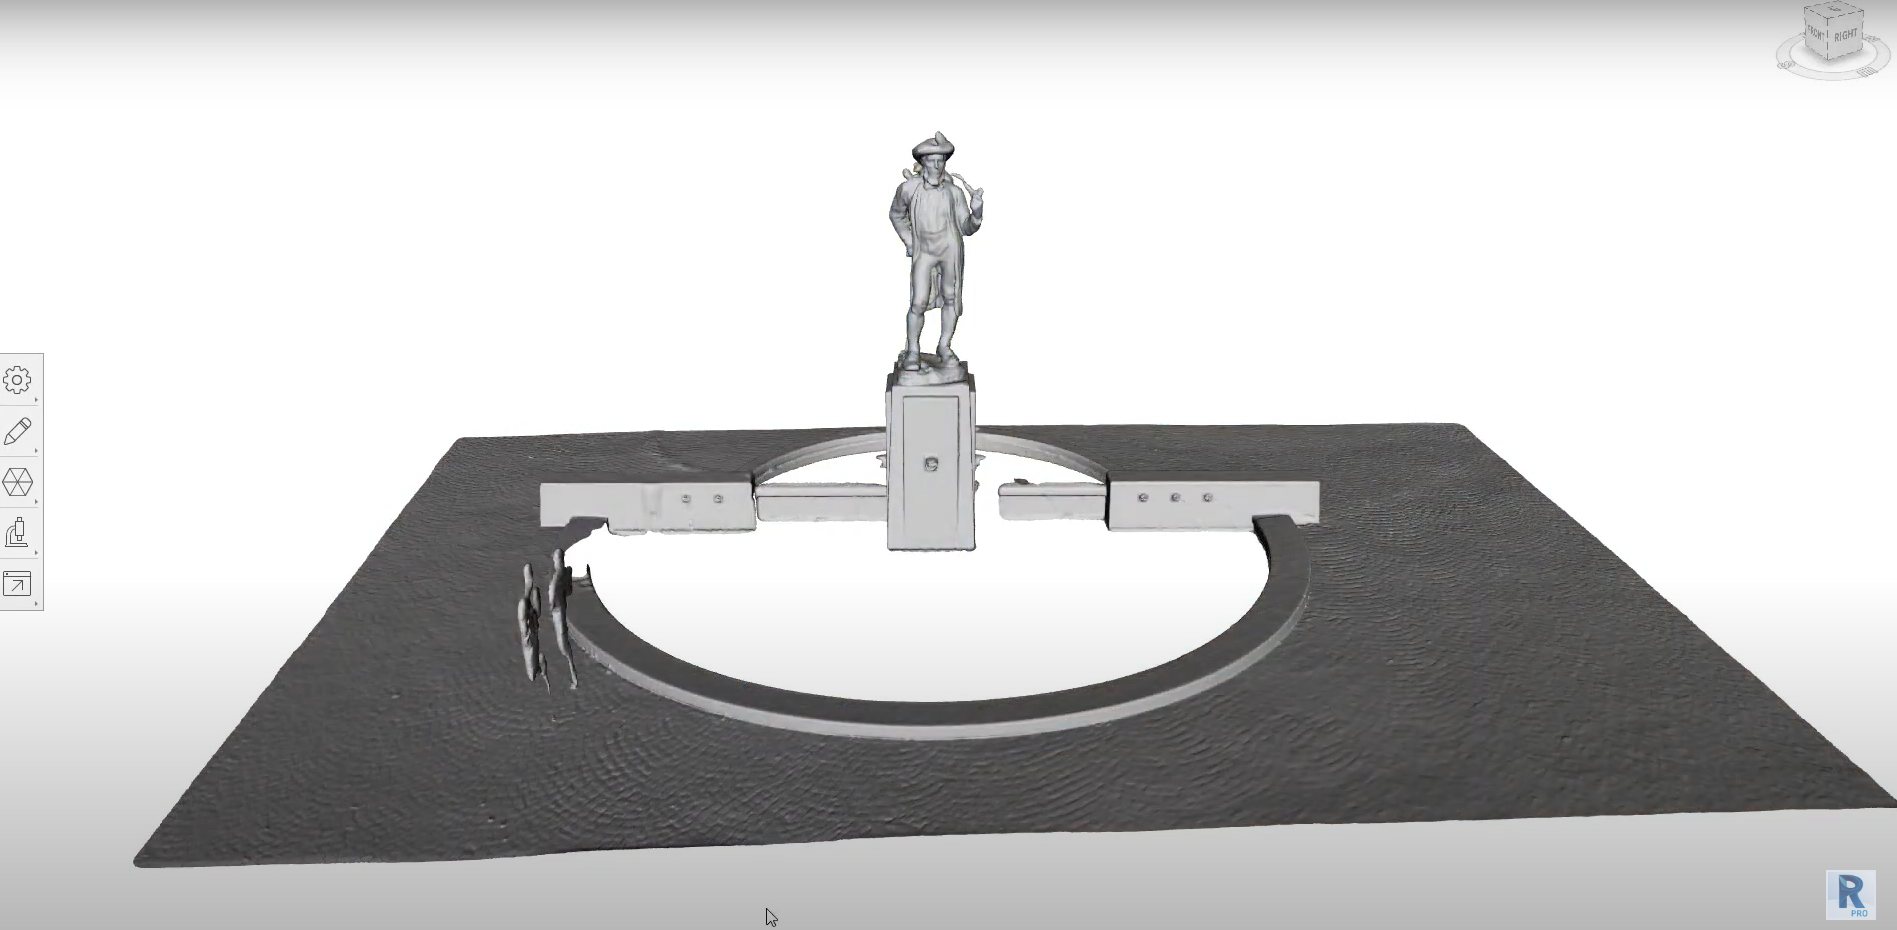
\includegraphics[width= 0.9\textwidth]{Figures/Finalmesh.PNG}
  \caption[Final Mesh]{Final Mesh}
\end{figure}
\noindent Now by this model, architectures can make a CAD model for 3D reconstruction.
\section{Point Cloud of Scanned Hallway}
After processing the scanned data with Agisoft Metashape software we get point cloud of hallway which showed in Figure \ref{fig:Hallway pointcloud}.

\begin{figure}[H]
  \centering
  \subfloat[Hallway point cloud from front view.]{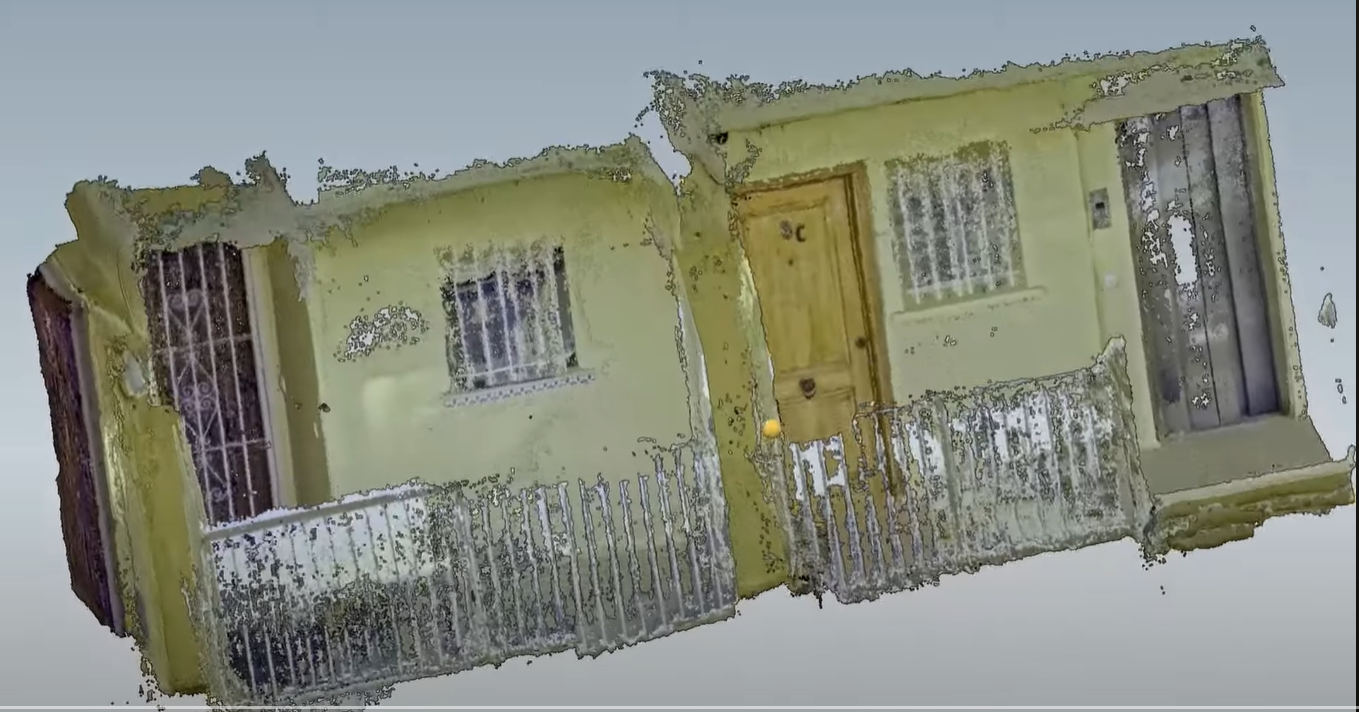
\includegraphics[width=0.9\textwidth]{Figures/hallscan.PNG}\label{fig:hallscan}}
  \hfill
  \subfloat[Hallway entrance point cloud visualized in Blender software.]{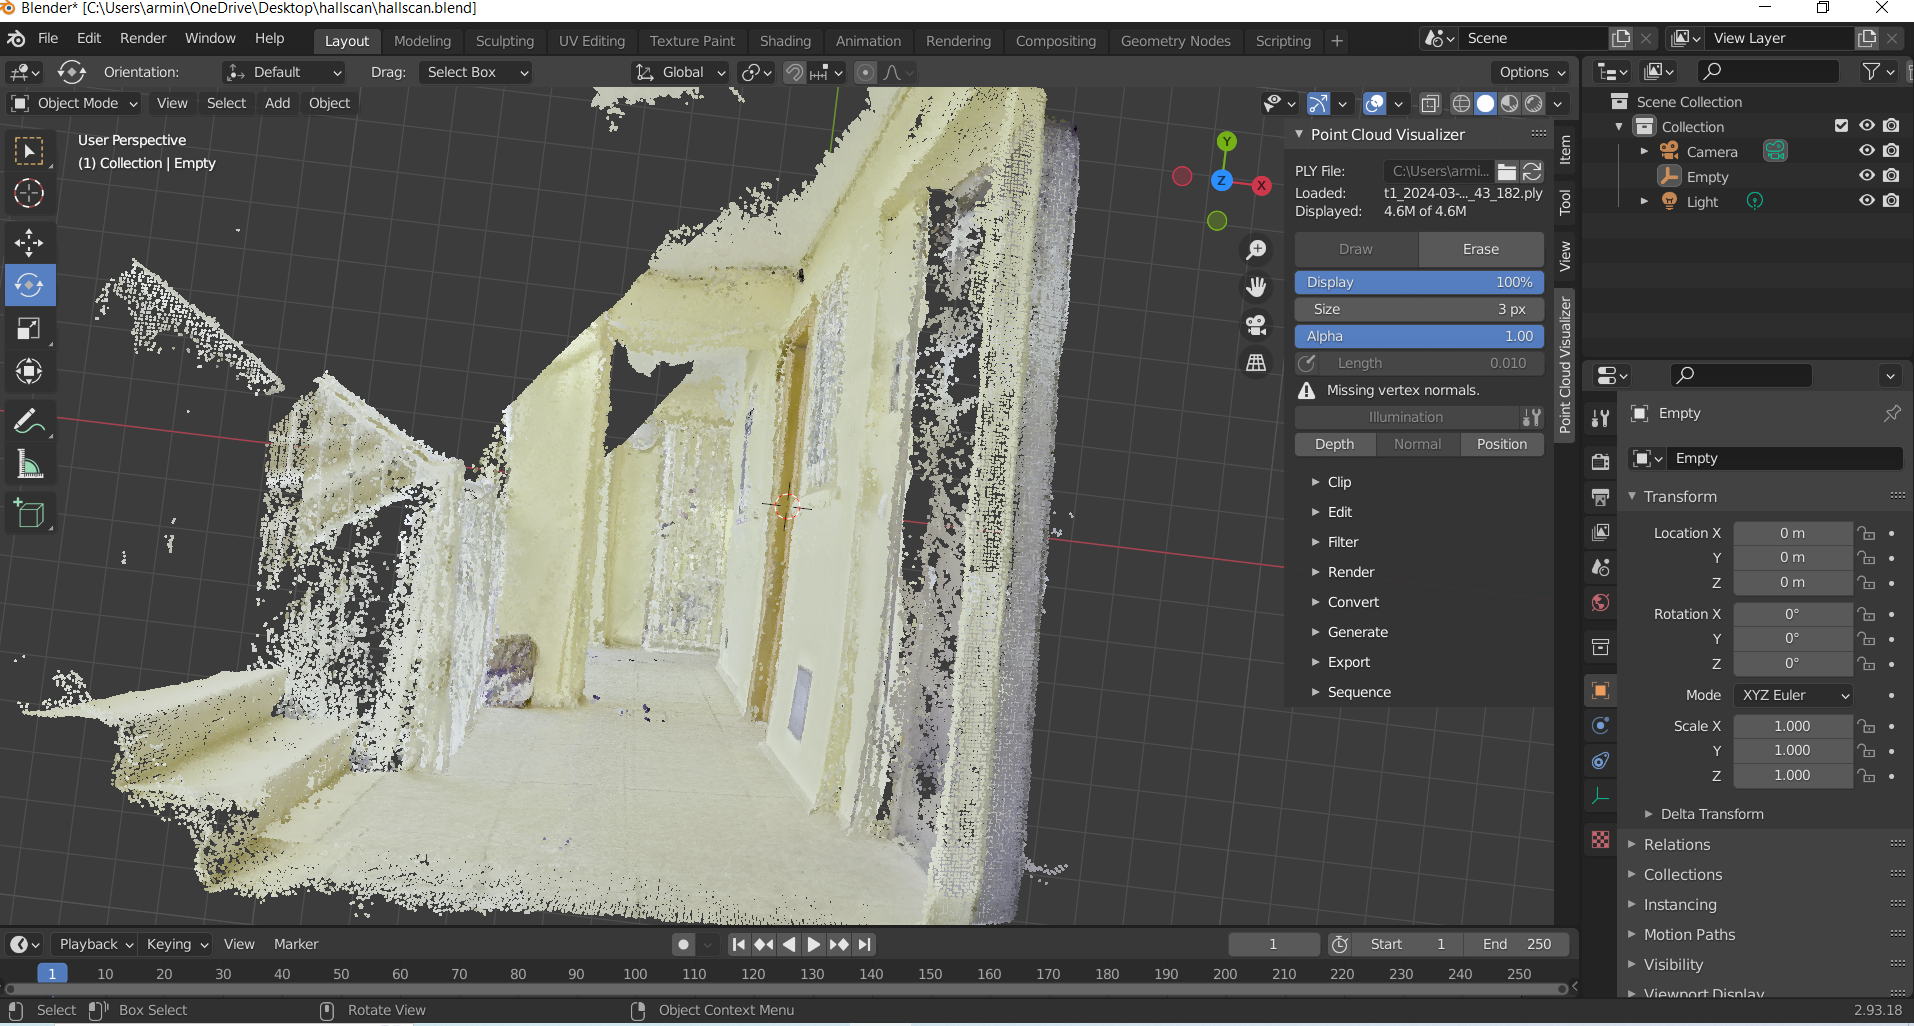
\includegraphics[width=0.9\textwidth]{Figures/Blender file of corridoor scan.PNG}\label{fig:Hallway point cloud in Blender}}
  \hfill
  \subfloat[Hallway point cloud from closer view.]{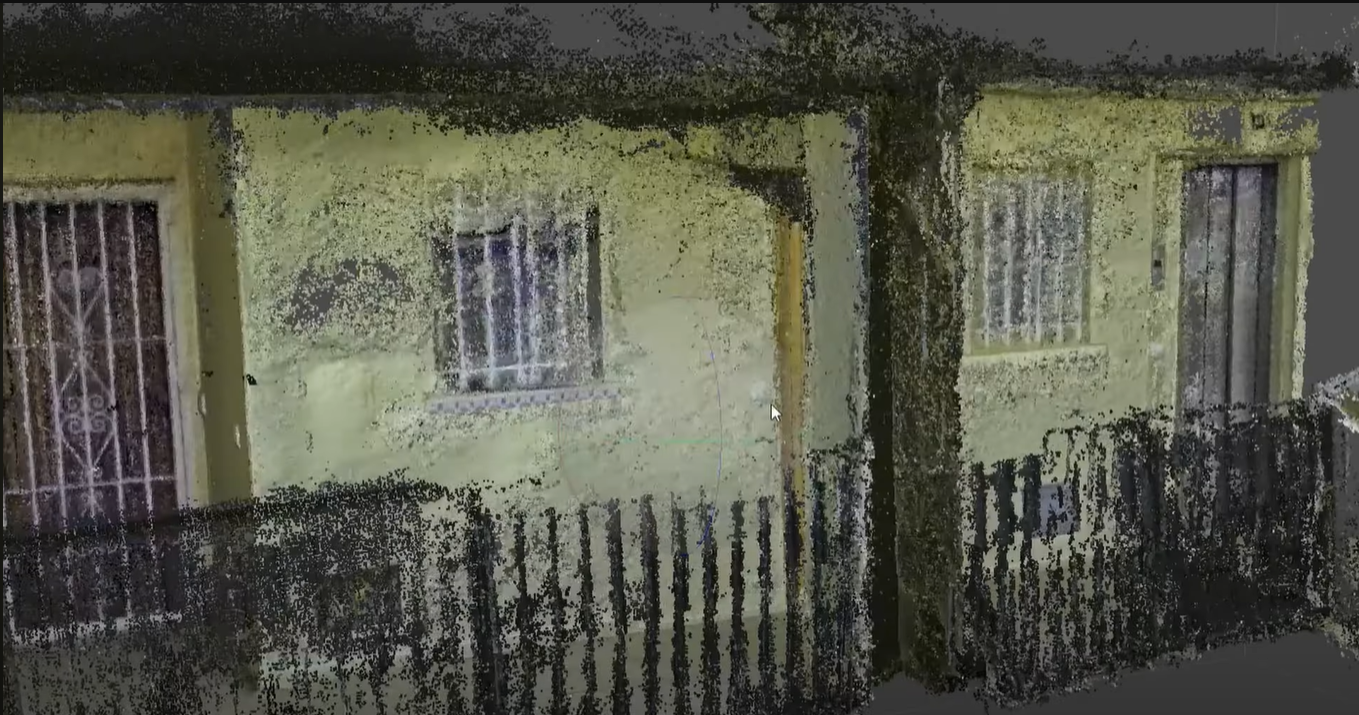
\includegraphics[width=0.8\textwidth]{Figures/hallscan1.PNG}\label{fig:Hallway point cloud from close view}}
  
  \caption[Hallway point cloud from closer view]{Figure (a) shows the point cloud from front view, figure (b) shows the start of scanning location and its point cloud, and figure (c) shows the point cloud from closer view.}
\label{fig:Hallway pointcloud}
\end{figure}

\noindent Next step is adding mesh to the point cloud with Cloud Compare. As it is shown in Figure \ref{fig:Hallway with Mesh} the mesh is added to the point cloud of hallway.
\begin{figure}[H]
  \centering
  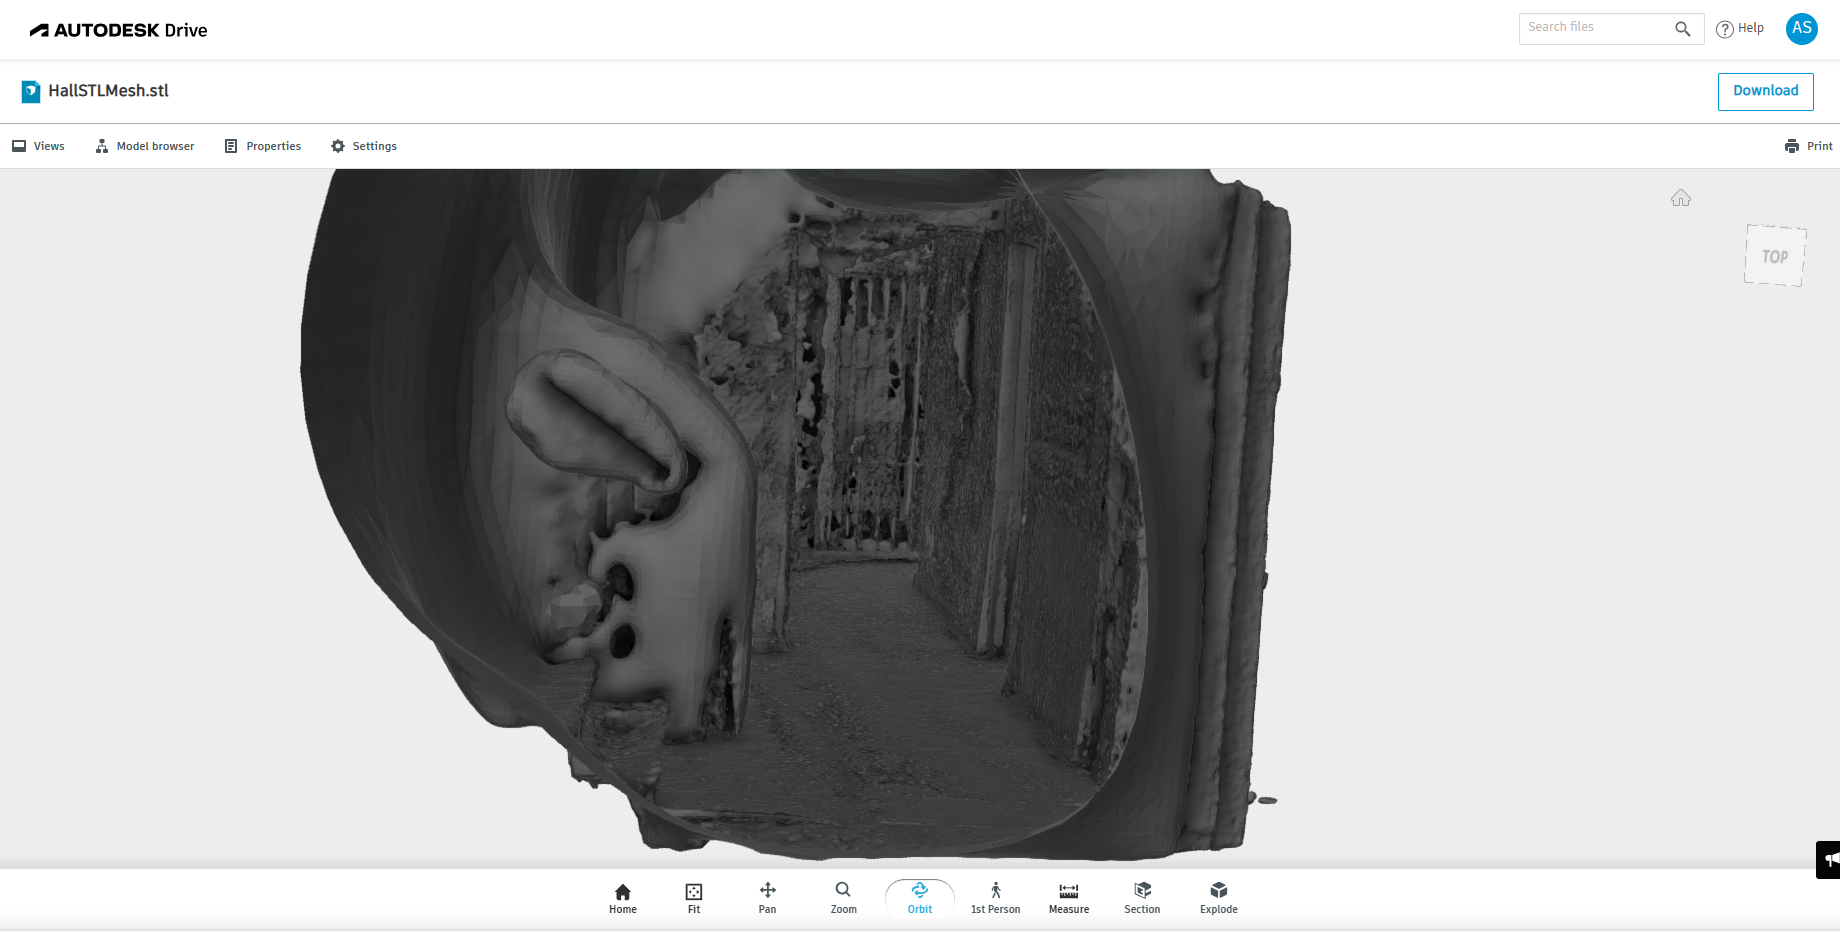
\includegraphics[width= 1.0\textwidth]{Figures/Meshhall.PNG}
  \caption[Picture of Meshed Hallway]{Picture of hallway with mesh}
  \label{fig:Hallway with Mesh}
\end{figure}
Now my meshed hallway is ready to be imported to the Coppeliasim software for simulation, after import I decided to simulate behaviour of an UGV (Unmanned Ground Vehicle) called "Pioneer p3dx" with two different algorithms and environment. The environment is shown in Figure
\ref{fig:Path visualization of pioneer p3dx}.

\begin{figure}[H]
  \centering
  \subfloat[Virtual indoor environment in CoppeliaSim]{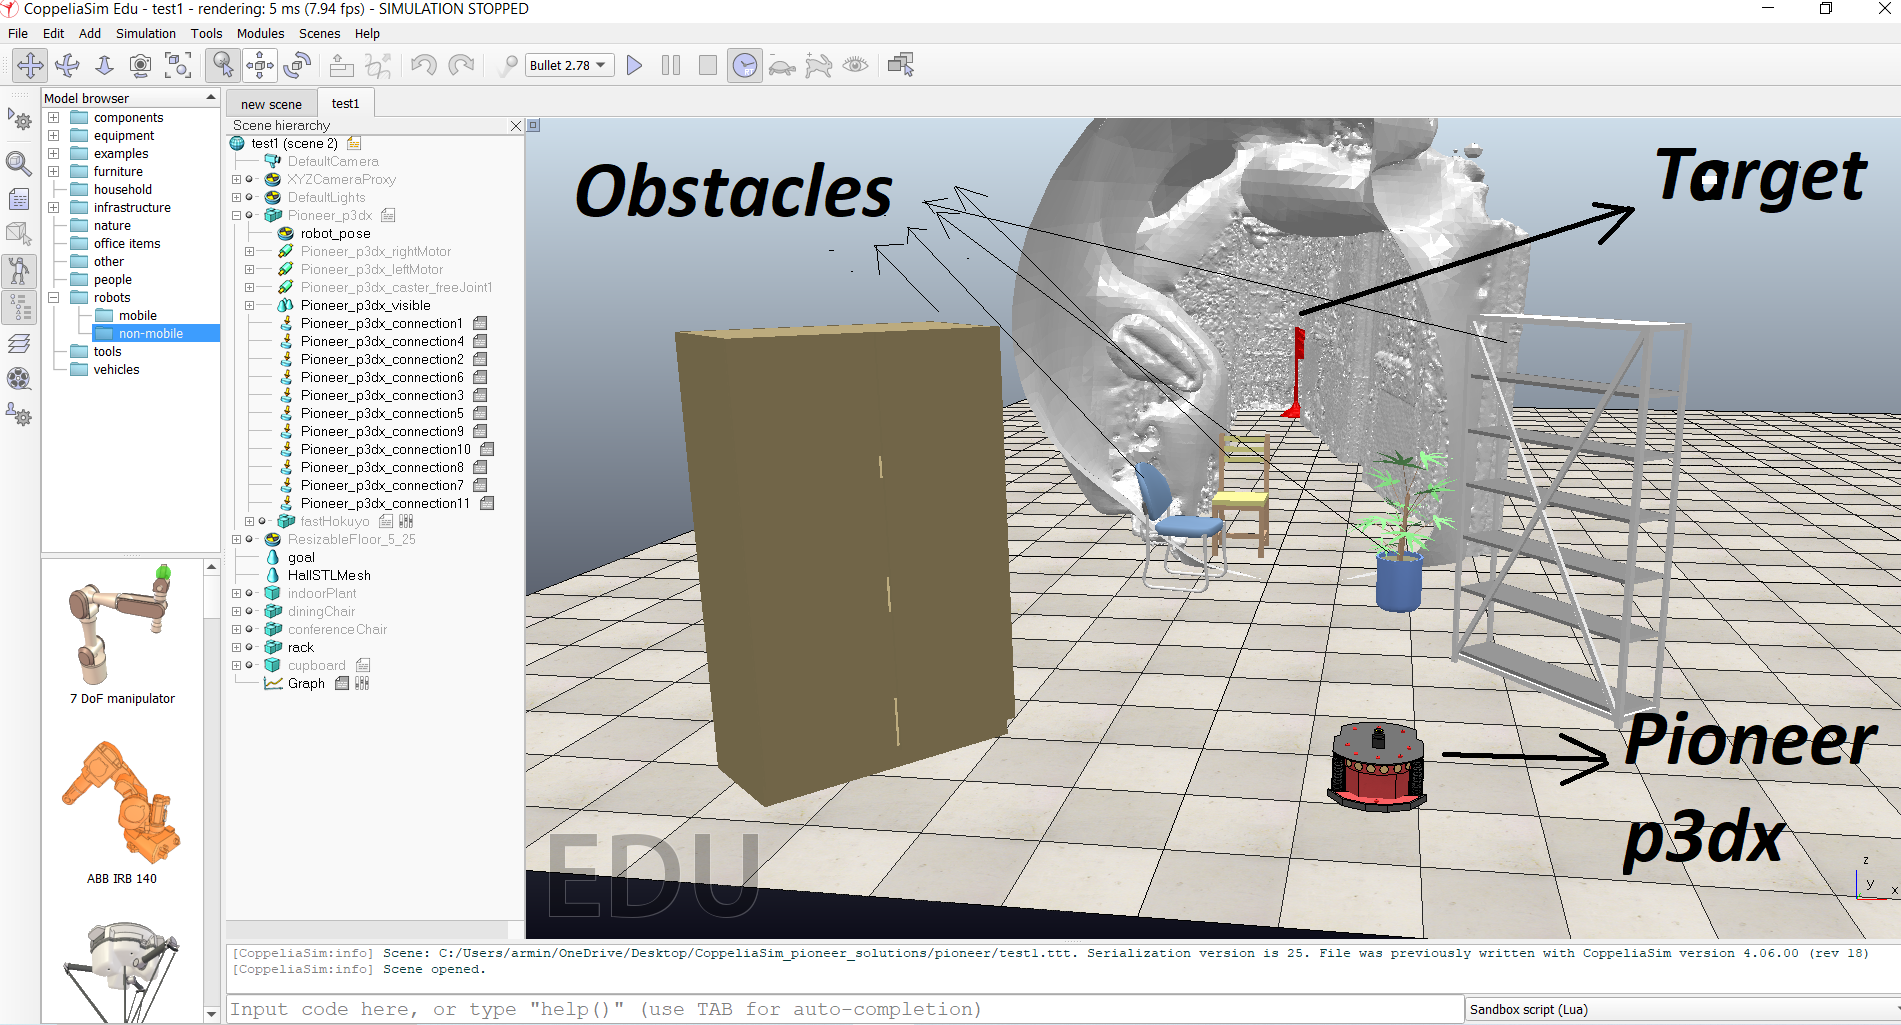
\includegraphics[width=0.9\textwidth]{Figures/Indoor environment.PNG}\label{fig:CoppeliaSim Virtual Environment}}
  \hfill
  \subfloat[Coordination of virtual environment]{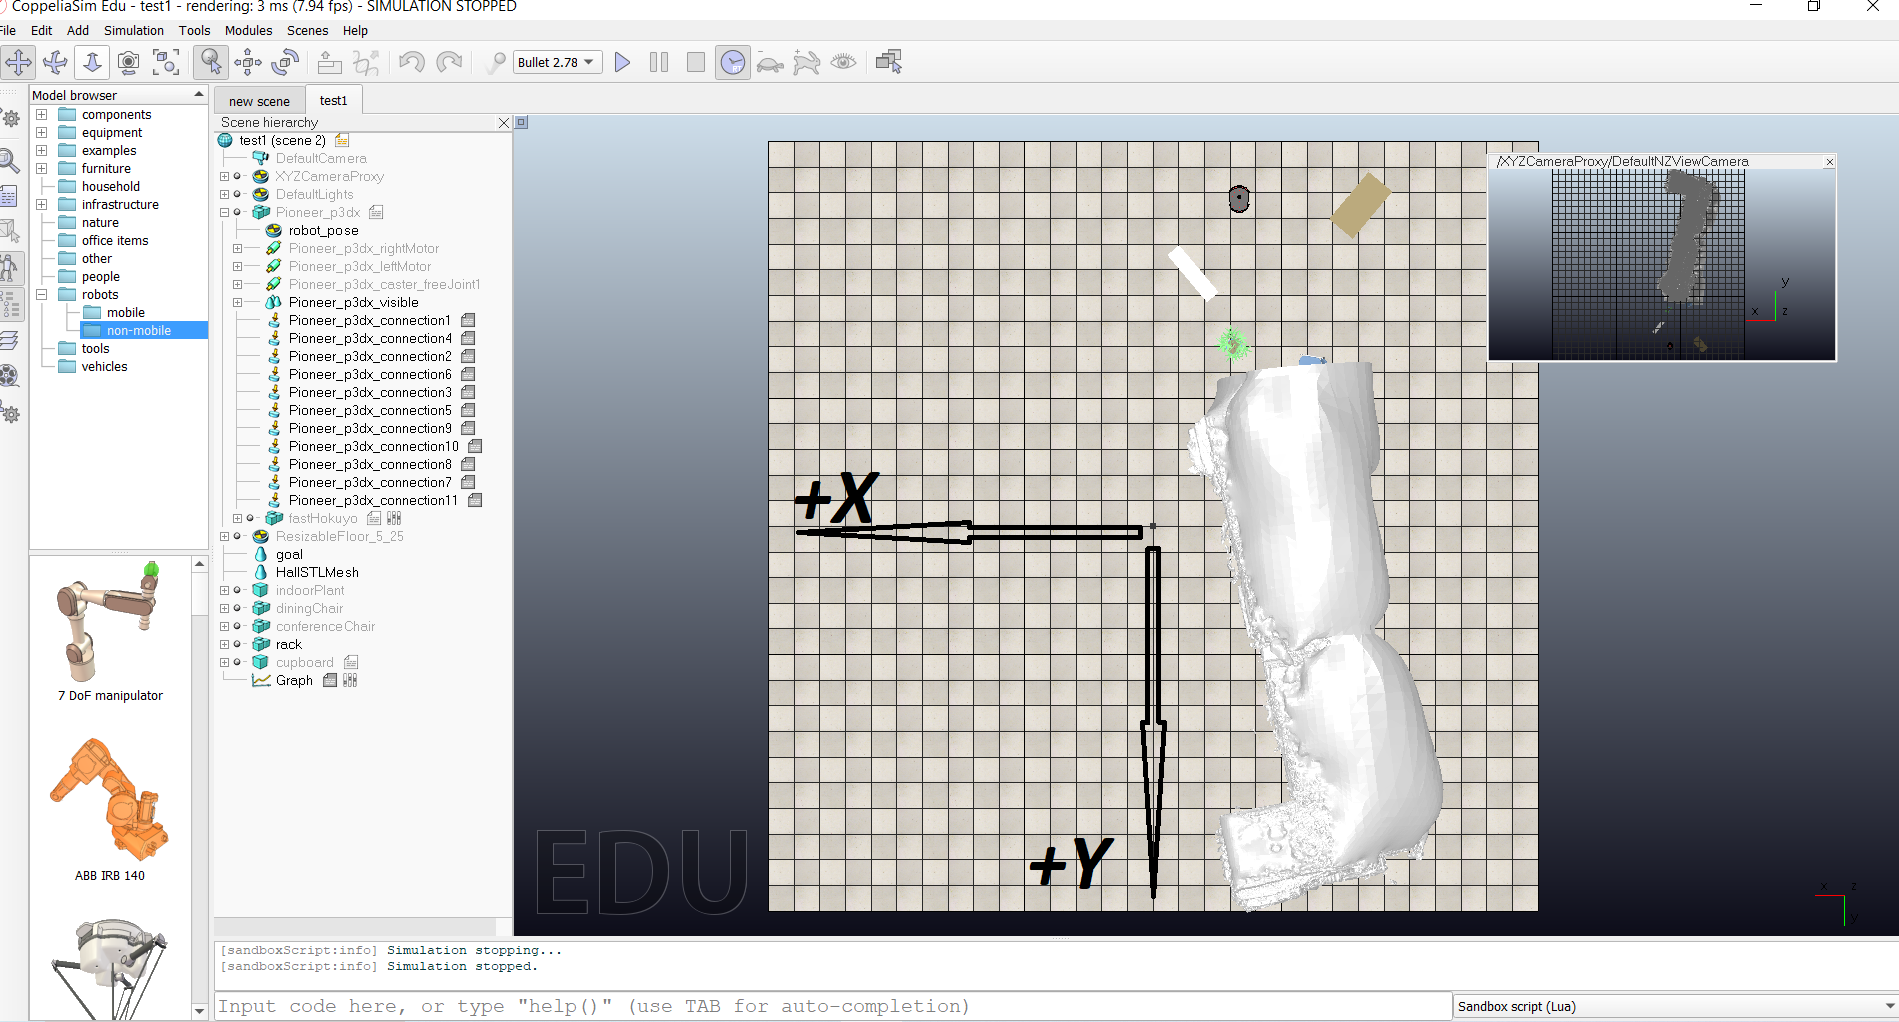
\includegraphics[width=0.7\textwidth]{Figures/Coordinate in Copppelia.PNG}\label{fig:CoppeliaSim Coordination}}
  \hfill
  \subfloat[Path and velocity direction graph of Pioneer p3dx after goal tracking]{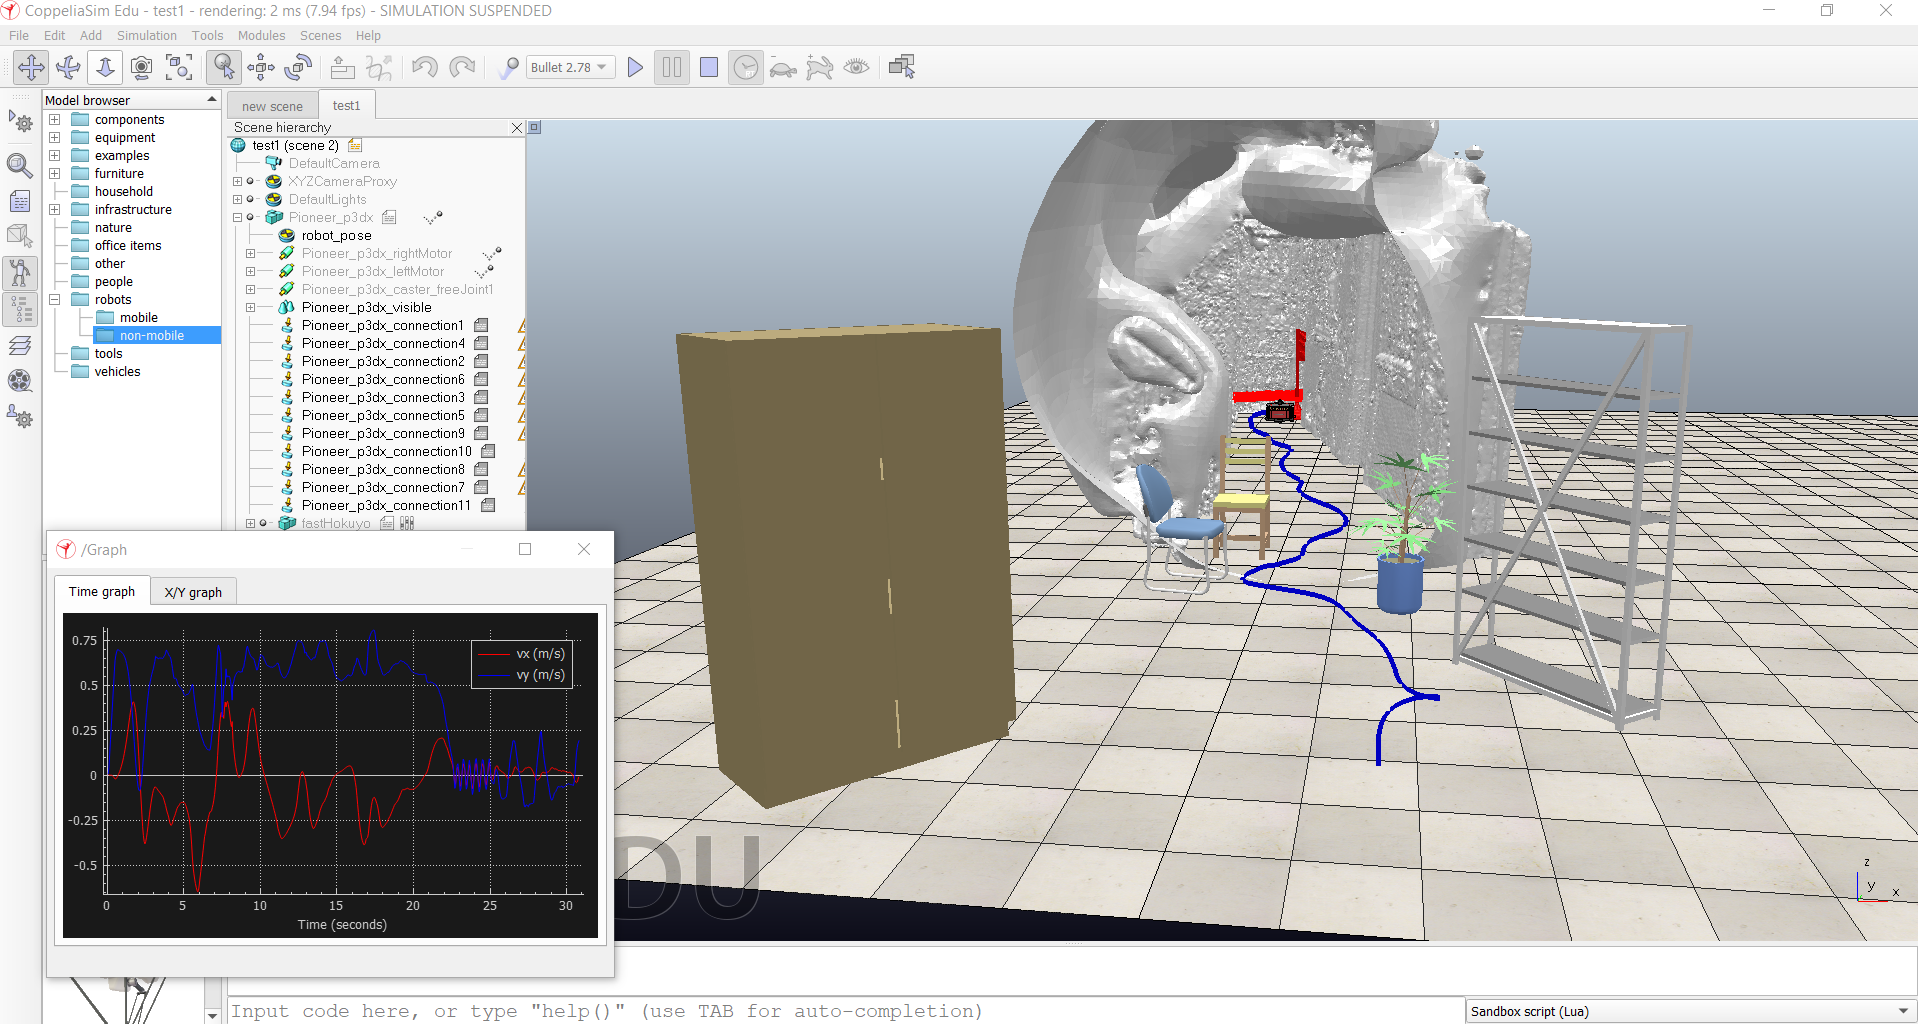
\includegraphics[width=1\textwidth]{Figures/Path and Velocity direction graph.PNG}\label{fig:Path visualization of pioneer p3dx}}
  
  \caption[Simulation in CoppeliaSim]{Figure (a) Shows a virtual environment based on the imported mesh , figure (b) shows coordination in the CoppeliaSim, and figure (c) shows path and velocity direction of the Pioneer p3dx.}
\label{fig:Path visualization of pioneer p3dx}
\end{figure}



\section{Point Cloud in Shipbuilding Sector}

First it was planned to scan a ship with 360 degree camera for point cloud generation, but due to confidentiality of projects, it was not possible.So I decided to find a Pre-made point cloud of a ship Called SY Carola from Scottish Maritime Museum. SY Carola is possibly the world's oldest seagoing steam yacht. Scott and Sons of Bowling built it in 1898 at their shipyard on the Clyde River's north bank. Carola is 70 feet long and made of steel, with teak decking and a deckhouse. She presently has two masts.
Carola, built for personal use by the shipbuilder's family, served as a yacht during the summer months and, when not in use by the family, took groups of senior yard staff on Clyde excursions. In the winter, it would have been used as a tender and tug at the shipyard.By 1964, it had been sold to a private owner before being purchased by a Sussex corporation in 1981 and converted into corporate hospitality.
Carola joined the Scottish Maritime Museum's collection in 1994.
The model was developed as part of the 'Scanning The Horizon' 3D digitisation project\cite{Carolaship}. In Figure \ref{fig:SY Carola point cloud} the Carola point cloud is shown. 

\begin{figure}[H]
  \centering
  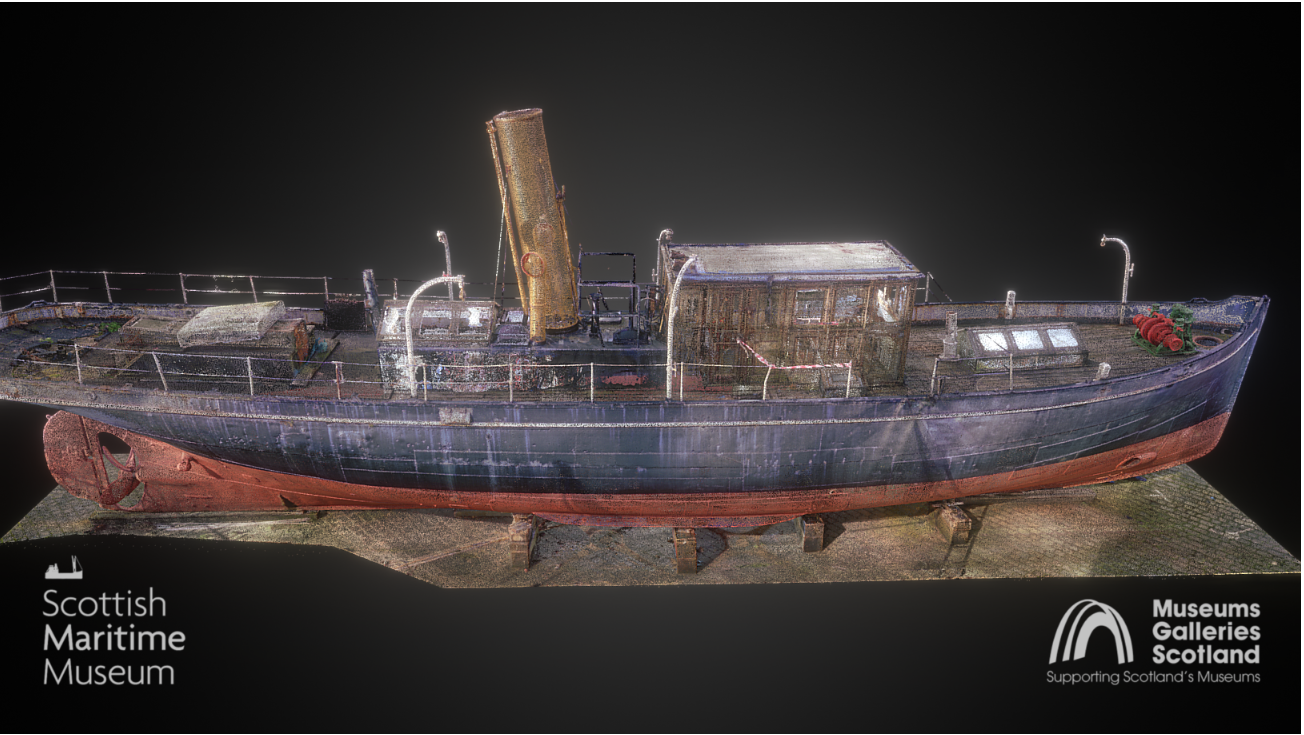
\includegraphics[width= 0.9\textwidth]{Figures/Crolaship.PNG}
  \caption[Picture of Visualized SY Carola Point Cloud]{Picture of SY Carola point cloud} \cite{Carolaship}
   \label{fig:SY Carola point cloud}
\end{figure}
\noindent After that I tried to import the point cloud to the CoppeliaSim for robot simulation on the deck but, the imported point cloud was black and not suitable as a virtual environment, although the the point cloud was detectable, collidable and measurable by the virtual robot. In figure \ref{fig:SY Carola point cloud} the imported point cloud to the CoppeliaSim is shown. 
\begin{figure}[H]
  \centering
  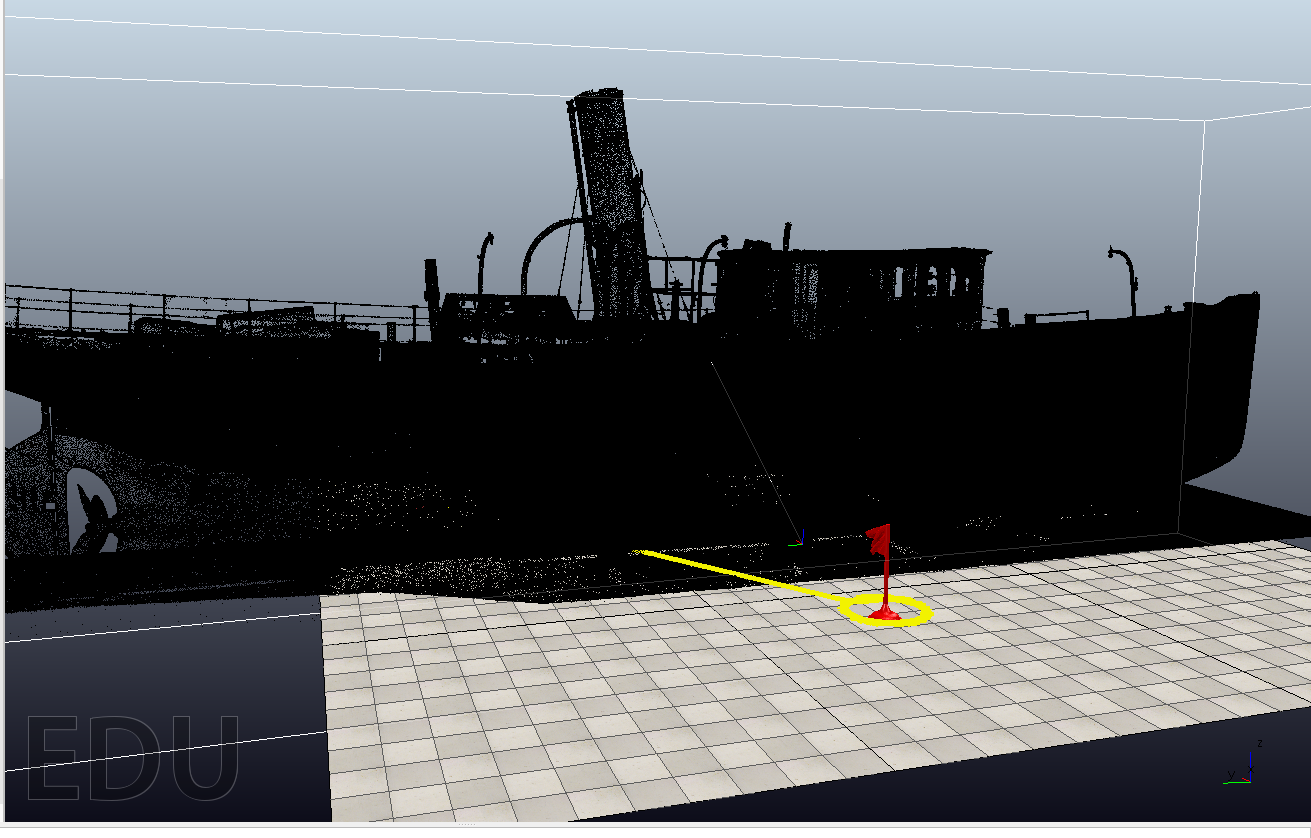
\includegraphics[width= 0.8\textwidth]{Figures/ship point clould in Coppeliasim.PNG}
  \caption[Picture of SY Carola Point Cloud in CoppeliaSim]{Picture of SY Carola point cloud in CoppeliaSim}
   \label{fig:Carola point cloud in CoppeliaSim}
\end{figure}
\noindent So then I tried to use mesh of Carola ship to import to the CoppeliaSim. As it is shown in Figure \ref{fig:Mesh of SY Carola in Autodesk}. 
\begin{figure}[H]
  \centering
  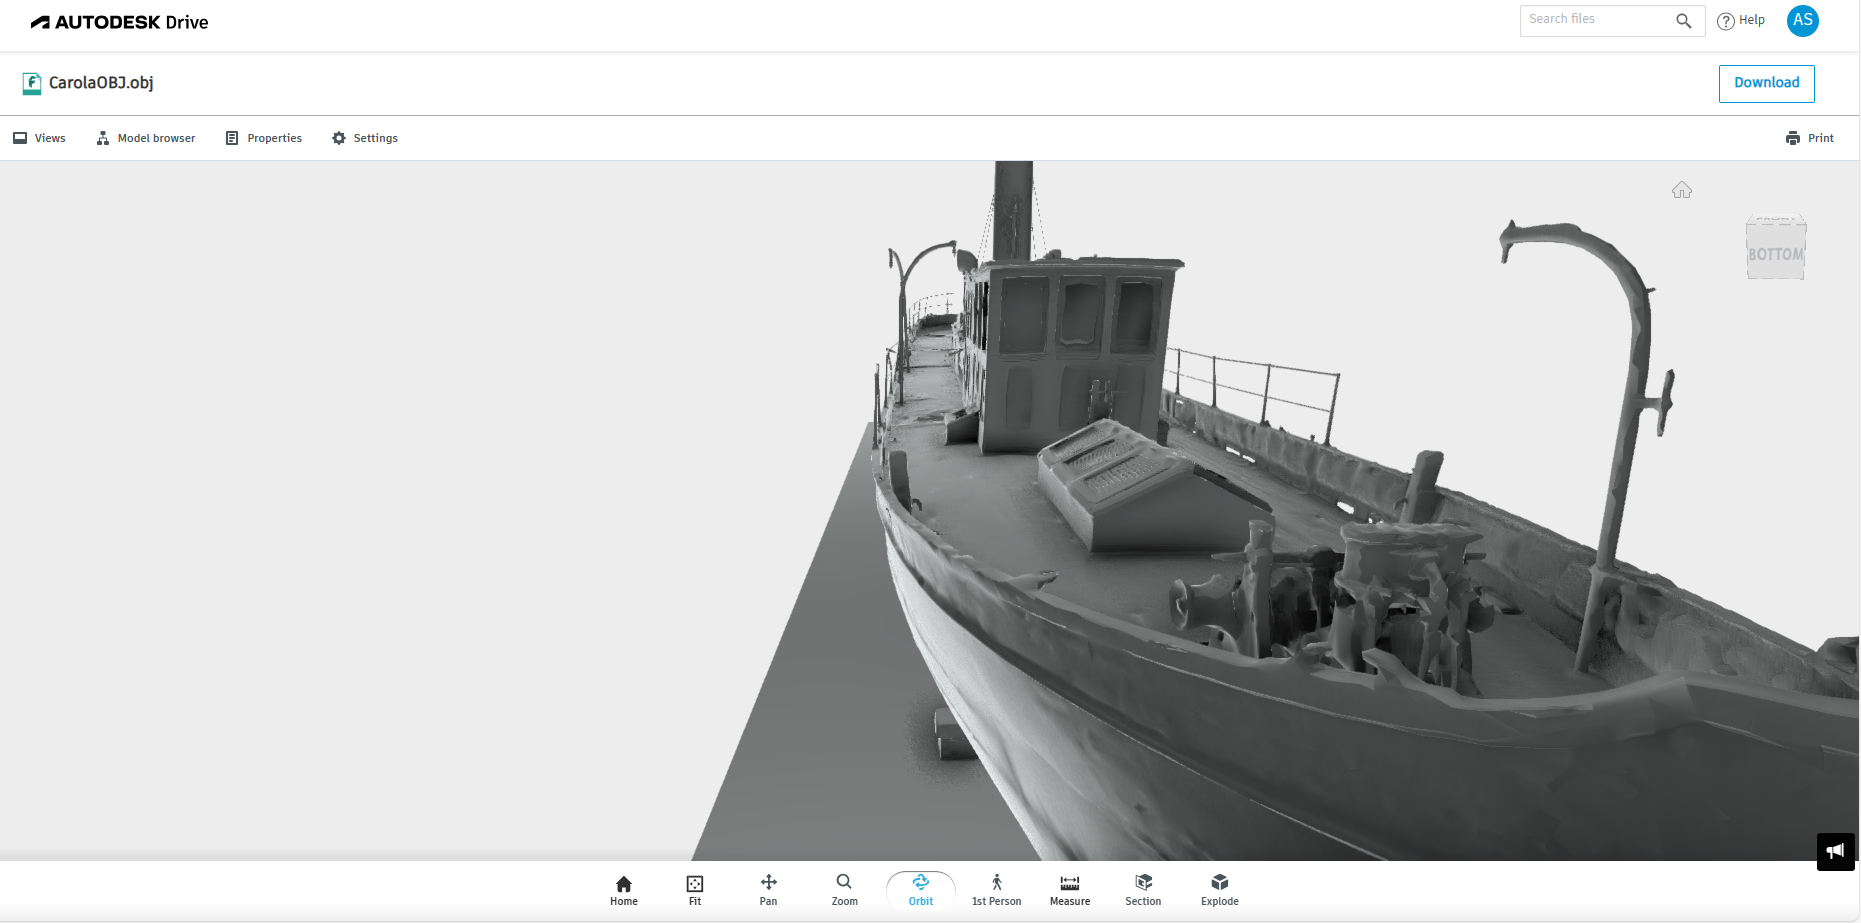
\includegraphics[width= 0.9\textwidth]{Figures/Carola mesh.PNG}
  \caption[Mesh of SY Carola in Autodesk]{Mesh of SY Carola in Autodesk}
   \label{fig:Mesh of SY Carola in Autodesk}
\end{figure}

\noindent But due to less-complexity of Carola,s deck obstacles for robot simulation, I selected a ship with complex deck design.The imported mesh is shown in Figure \ref{fig:Mesh of A Ship in CoppeliaSim}. 
\begin{figure}[H]
  \centering
  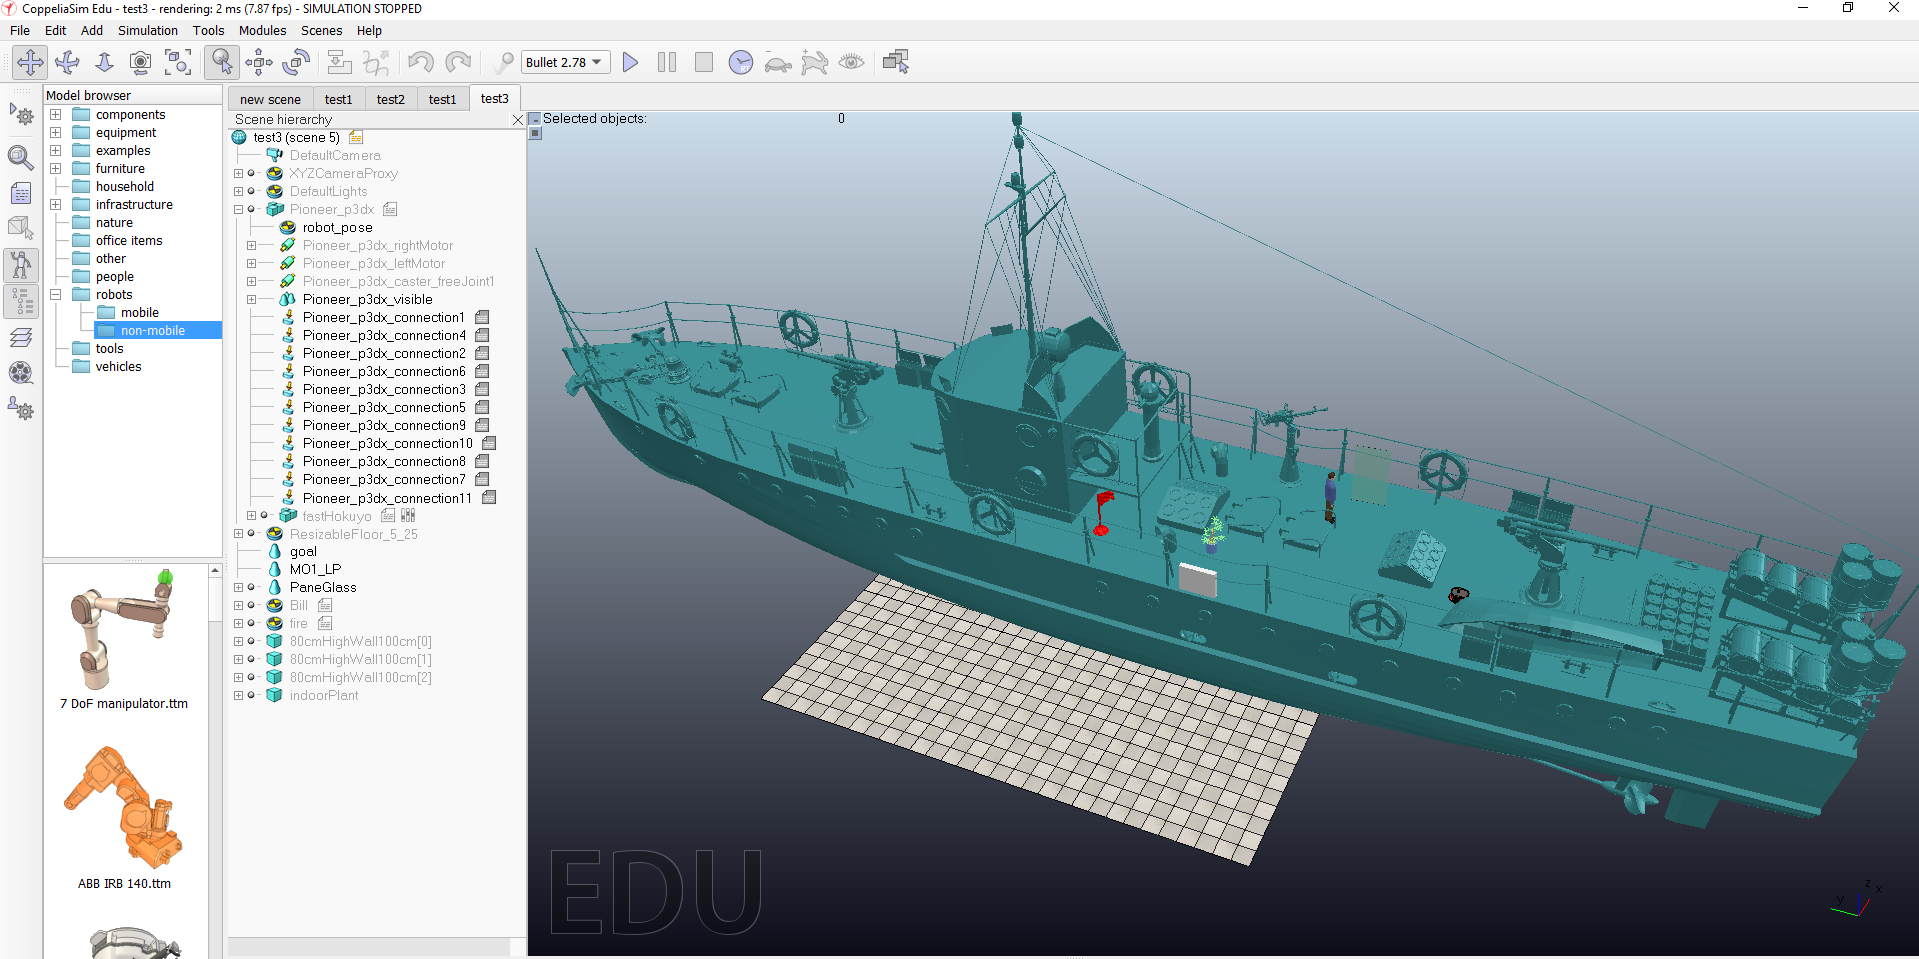
\includegraphics[width= 1.0\textwidth]{Figures/CoppeliaMesh.PNG}
  \caption[Mesh of A Ship in CoppeliaSim]{Mesh of A Ship in CoppeliaSim}
   \label{fig:Mesh of A Ship in CoppeliaSim}
\end{figure}



\section{Qualitative and Quantitative Results}
\noindent In this section I simulated Pioneer 3dx robot in my virtual environment with two prefabricated algorithms called: potential field and Vector Field Histogram Plus(VFH+). One of the virtual environments is an indoor place (scanned hall) and another one is an
outdoor environment (ship model). Two types of qualitative and quantitative results have been compared and investigated.
  
\subsection{Simulation With Pioneer 3dx Based on the Potential Field Method in a Scanned Hall Mesh (Indoor Environment) }
\noindent As you can see in the Figure \ref{fig:Indoor environment with scanned hall mesh} the robot is located between obstacles with different sizes and locations. The goal is at the end of scanned hall in right side which is source of attractive force in the environment.   
\begin{figure}[H]
  \centering
  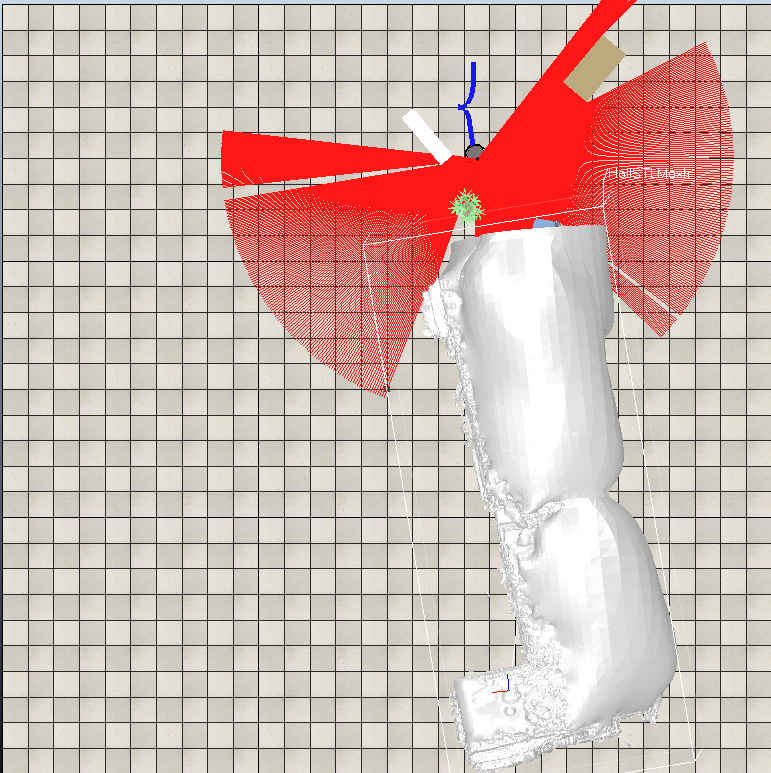
\includegraphics[width= 0.6\textwidth]{Figures/1.PNG}
  \caption[Indoor environment with scanned hall mesh]{Indoor environment with scanned hall mesh} 
   \label{fig:Indoor environment with scanned hall mesh}
\end{figure}

\noindent In the Figure \ref{fig:Obstacles in the scene without hidden scanned hall mesh} it is shown the environment with hidden hall mesh to be clear about the place of obstacles and goal.  

\begin{figure}[H]
  \centering
  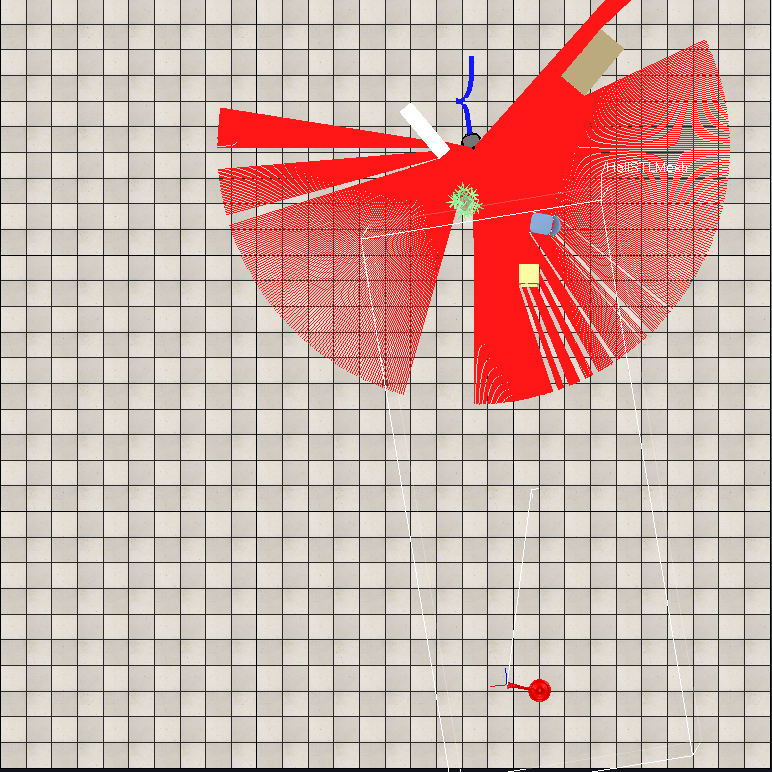
\includegraphics[width= 0.6\textwidth]{Figures/2.PNG}
  \caption[Obstacles in the scene without hidden scanned hall mesh]{Obstacles in the Scene without hidden scanned hall mesh}
   \label{fig:Obstacles in the scene without hidden scanned hall mesh}
\end{figure}
After testing the robot in different environment arrangement, it found that in the following arrangement the robot will be trapped: 


\begin{itemize}
      \item  \textbf{ U-shape Obstacles or Concave Obstacles: }\\
      The robot can be trapped in u-shape or concave geometries due to local minimum specifically when the robot is far from the goal.   
      A polygon is convex if its inner angles are all fewer than 180 degrees. If one or more internal angles exceed 180 degrees, the polygon is non-convex (or concave). In Figure \ref{fig:Concave polygon and U-shape Obstacle} shown the two obstacles with repulsive forces around, one is u-shape and another one is a concave polygon which the possibility of trapping the robot is high. 
\begin{figure}[H]
  \centering
  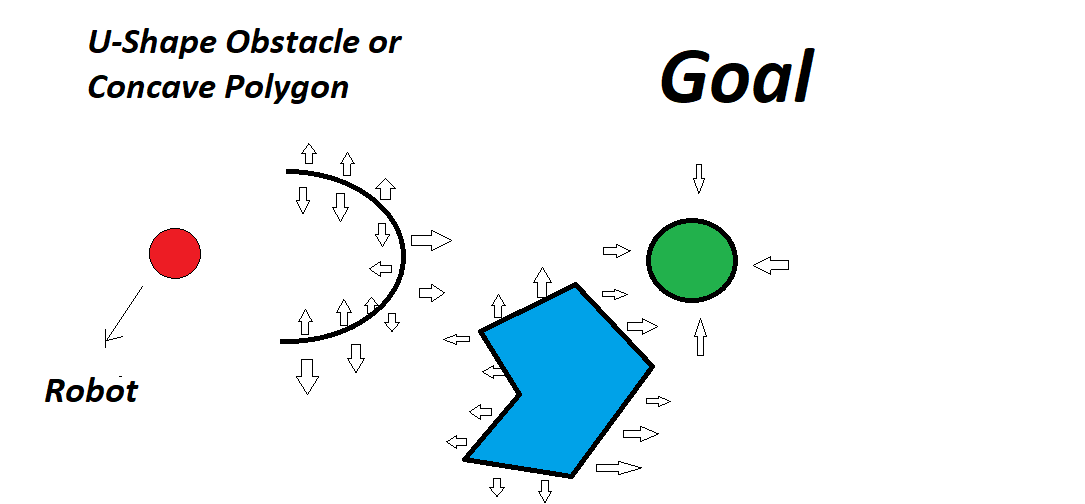
\includegraphics[width= 0.8\textwidth]{Figures/Concave polygon and U-shape.png}
  \caption[Concave polygon and U-shape Obstacle]{Concave polygon and U-shape Obstacle}
   \label{fig:Concave polygon and U-shape Obstacle}
\end{figure}
       \item  \textbf{ Oscillatory Behavior Between Obstacles: }\\
       In potential field method , there is a problem of oscillatory behavior of robot when the step size is too large. This issue happens when repulsive forces can be significantly higher than the attractive one which can cause the robot not to pass between obstacles even if physically could be possible. In Figure \ref{fig:Oscillatory Behavior} it is shown the situation that the robot stuck between a plant and hall structure.  
\begin{figure}[H]
  \centering
  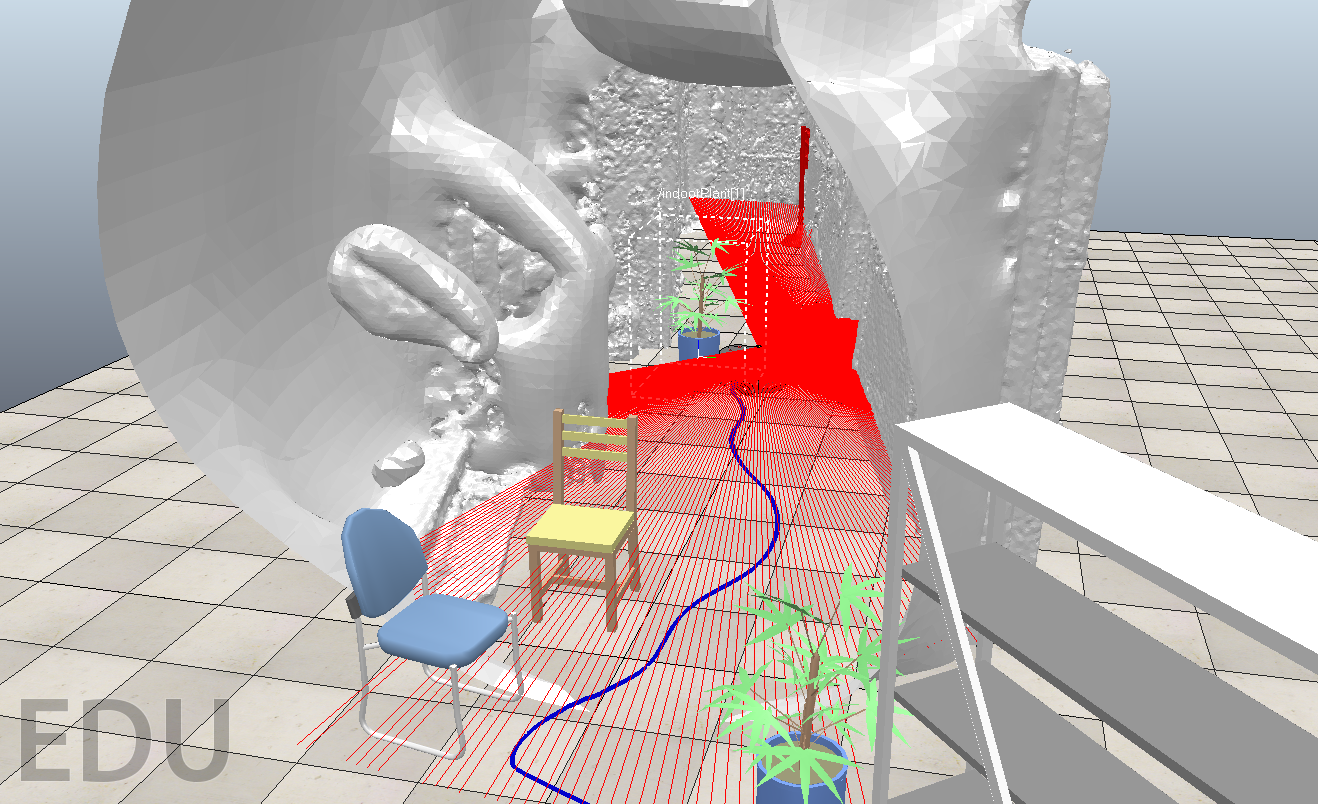
\includegraphics[width= 0.8\textwidth]{Figures/Oscillatory stuck.PNG}
  \caption[Oscillatory Behavior]{Oscillatory Behavior}
   \label{fig:Oscillatory Behavior}
\end{figure}

       
       \item  \textbf{ Crowded Obstacles : }\\
       In crowded areas, potential field approaches can cause the robot to become trapped. This is typically related to the formation of local minima in the potential field. As it is shown in the Figure \ref{fig:Crowd Obstacles} the summation of repulsive forces from obstacles are stronger than attractive force so the robot will stuck even if physically possible to pass the obstacles. 
\begin{figure}[H]
  \centering
  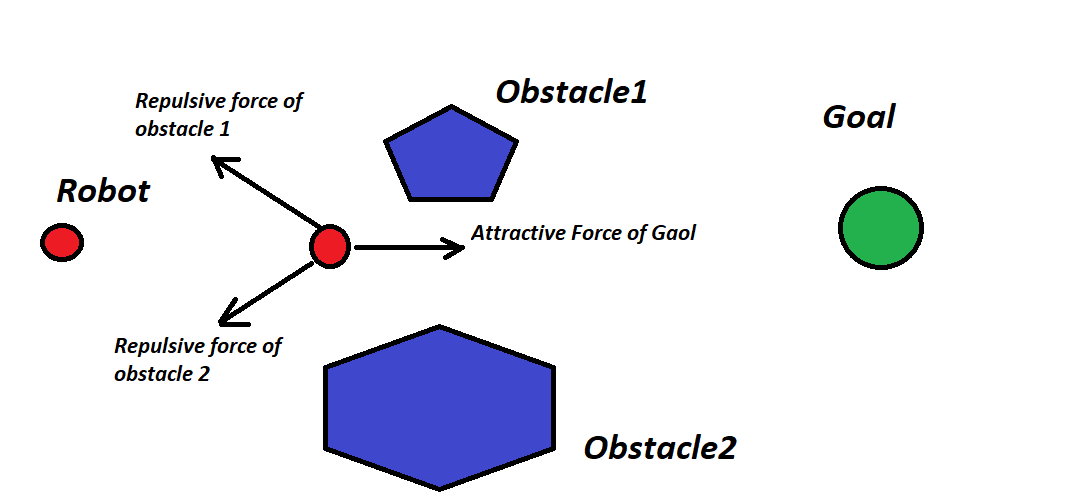
\includegraphics[width= 0.9\textwidth]{Figures/Crowd obstacles.png}
  \caption[Crowd Obstacles]{Crowd Obstacles}
   \label{fig:Crowd Obstacles}
\end{figure}

       
       \item  \textbf{ Less Detectable Obstacles: }\\
       The Artificial Potential Field (APF) method for robot path planning use a laser scanner to detect impediments. The robot perceives these impediments as sources of repulsive forces and attempts to maneuver around them. However, if the impediments are less noticeable or smaller than the threshold specified in the robot's programming, they may not be recognized as barriers. If a barrier is too small or not reflecting enough, the laser scanner may not detect it at all. This means that the robot will not recognize the impediment and may collide with it. Even if a little barrier is recognized, its repulsive force may not be sufficient to deflect the robot, particularly if the robot is moving quickly. As an example in our environment, legs of chairs are less detectable obstacles, an shown in Figure \ref{fig:Chair legs as less detectable obstacles}.   
\begin{figure}[H]
  \centering
  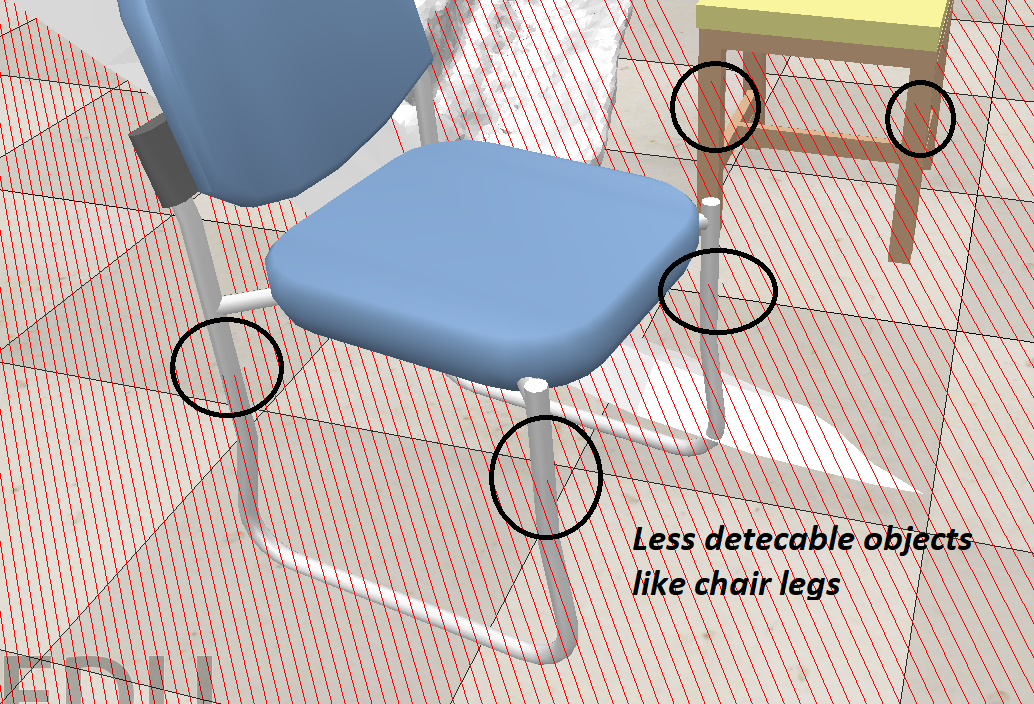
\includegraphics[width= 0.7\textwidth]{Figures/Chair legs.PNG}
  \caption[Chair legs as less detectable obstacles]{Chair legs as less detectable obstacles}
   \label{fig:Chair legs as less detectable obstacles}
\end{figure}

       \item  \textbf{ Height of Obstacles Which are Lower or Higher Than Laser Sensor Height : }\\
       The Artificial Potential Field (APF) method for robot path planning use a laser scanner to detect impediments. However, obstructions that are higher or lower than the laser scanner level can be difficult to navigate. If an obstacle is higher than the laser scanner's level, the scanner may be unable to identify it completely, especially if the barrier is close to the robot. This could result in erroneous mapping of the environment and possible collisions. Similarly, if an obstacle is below the level of the laser scanner, it may not be recognized at all. This is especially problematic for minor objects on the ground, which might lead the robot to trip or become trapped. A schematic view of this issue shown in Figure 
       \ref{fig:Higher and lower obstacles height than robot laser level}. 

\begin{figure}[H]
  \centering
  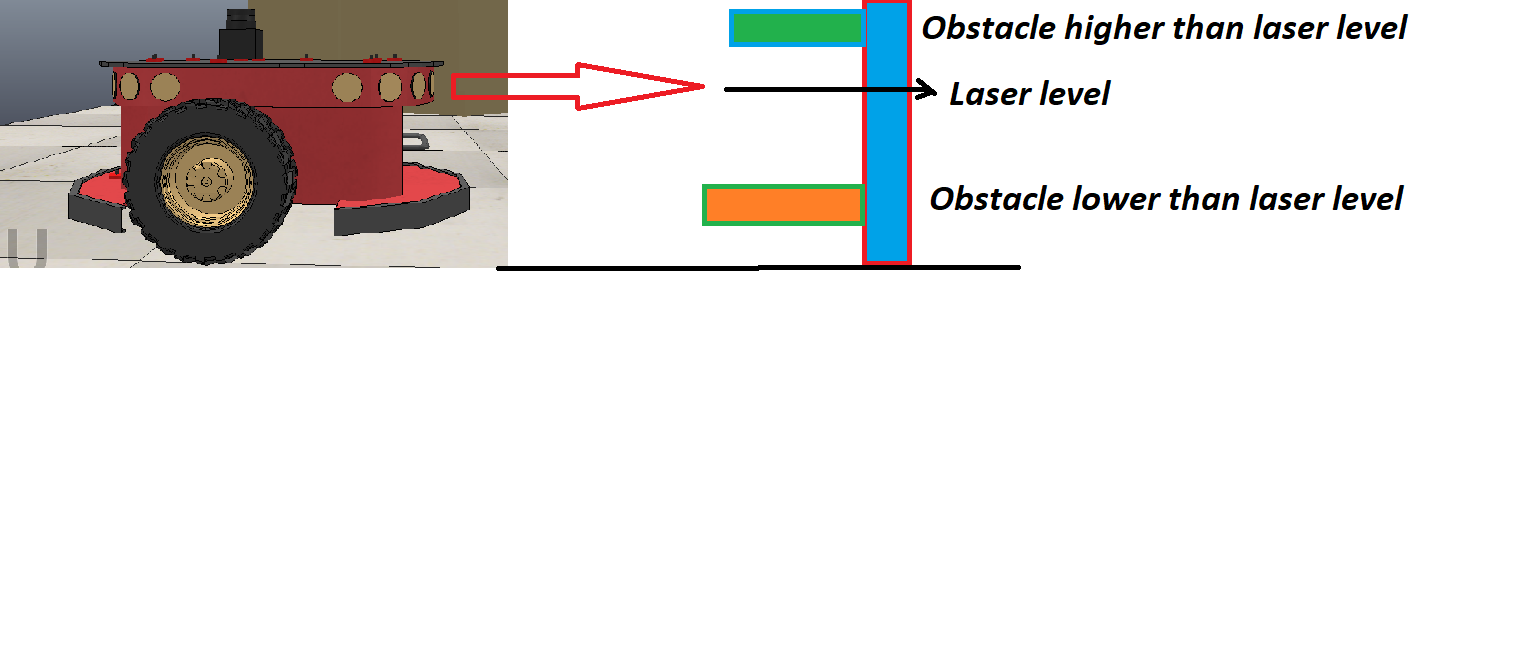
\includegraphics[width= 0.9\textwidth]{Figures/Laser level.png}
  \caption[Higher and lower obstacles height than robot laser level]{Higher and lower obstacles height than robot laser level}
   \label{fig:Higher and lower obstacles height than robot laser level}
\end{figure}
       
\end{itemize}




\subsection{Simulation With Pioneer 3dx Based on the Potential Field Method on the Deck of a Ship (Outdoor Environment) }
\noindent After importing the mesh or CAD model of a ship to the CoppeliaSim Software, I simulated a marine fire fighting operation with robot. Some items added to the scene to be more realistic like industrial robot, virtual fire and a flag. In Figure 
\ref{fig:Robot simulation on the deck of a ship for a short-range firefighting operation} it is shown the robot operation on the deck. This robot can autonomously navigate toward fire source if it does not trap. simulation has been done by adding more obstacles in the way of robot, or putting the robot back of an obstacle ,and it is seen that the likelihood of robot trapping is too much.  So it looks like potential field is better for short-range operation with less congested environment arrangement. \\
\begin{figure}[H]
  \centering
  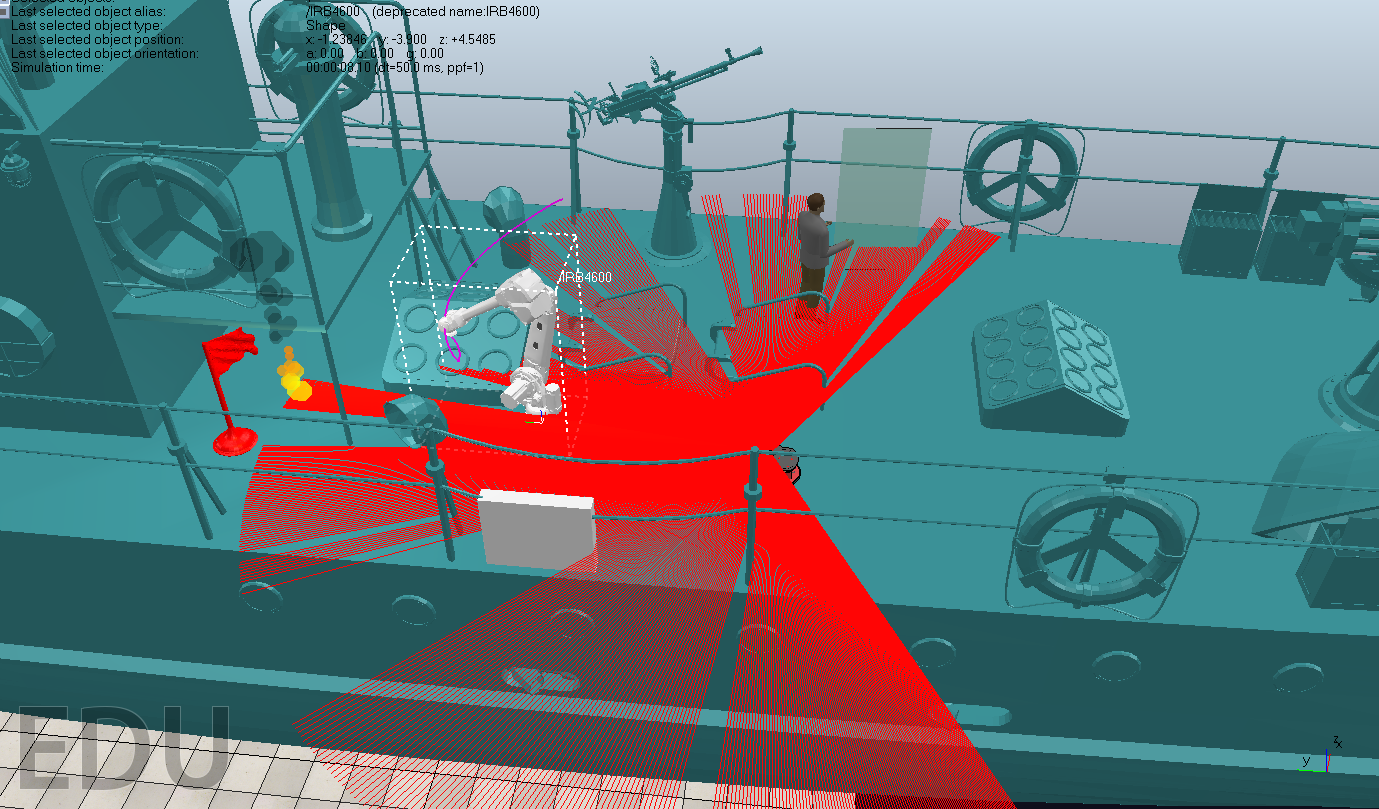
\includegraphics[width= 0.9\textwidth]{Figures/shipAPFSIM.PNG}
  \caption[Robot simulation on the deck of a ship for a short-range firefighting operation]{Robot simulation on the deck of a ship for a short-range firefighting operation}
   \label{fig:Robot simulation on the deck of a ship for a short-range firefighting operation}
\end{figure}

\subsection{Simulation with Vector Field Histogram Plus (VFH+) Method in an virtual Outdoor Environment with terrain) }

In this environment, robot surrounded by trees, scanned hall and terrains. Type of the terrains were implemented in this simulation was not complex terrains with lots of ups and downs. In Figure \ref{fig:Outdoor Environment for VFH+ Algorithm Simulation} the environment has been shown. 
\begin{figure}[H]
  \centering
  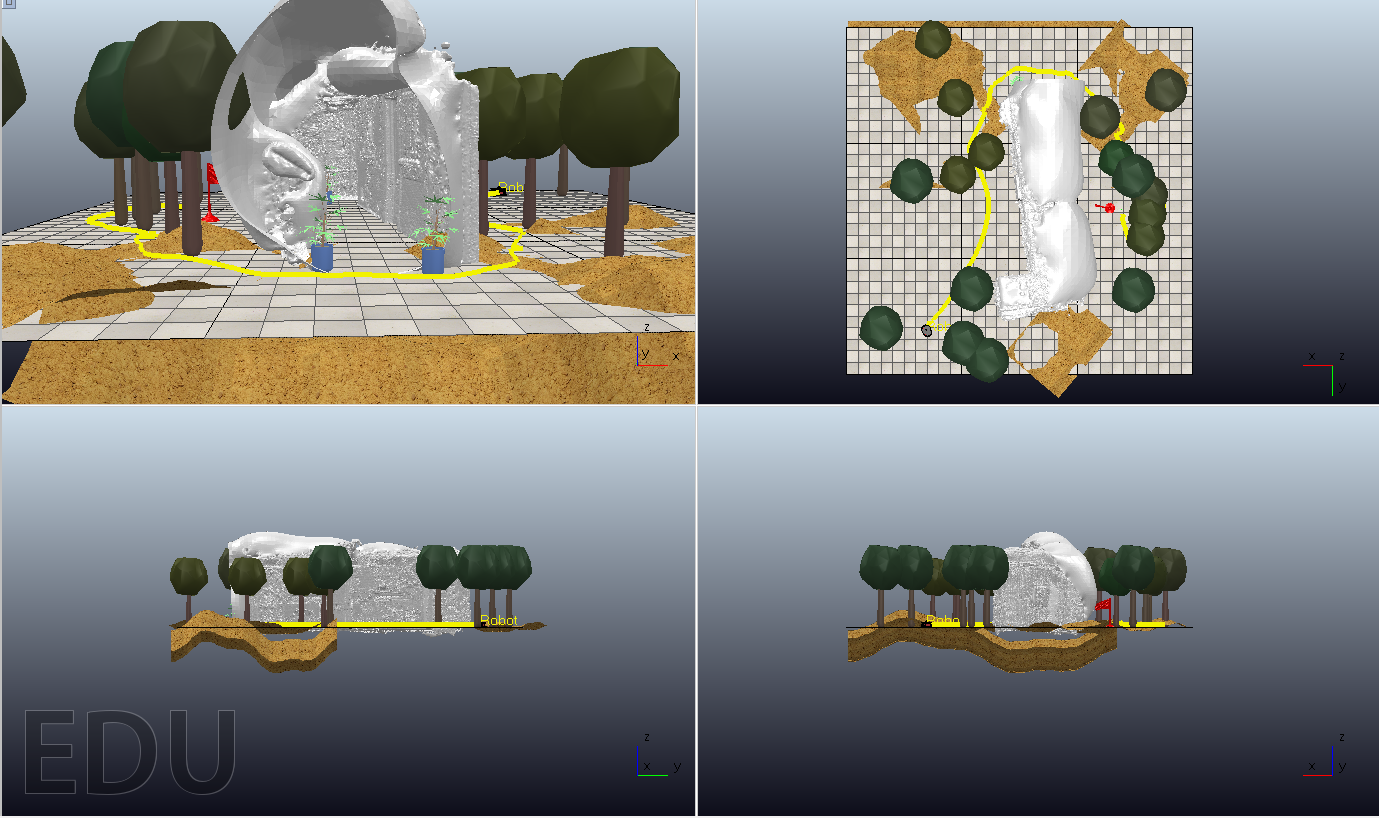
\includegraphics[width= 1.0\textwidth]{Figures/VFH+TERRAIN.PNG}
  \caption[Outdoor Environment for VFH+ Algorithm Simulation]{Outdoor Environment for VFH+ Algorithm Simulation}
   \label{fig:Outdoor Environment for VFH+ Algorithm Simulation}
\end{figure}
\noindent In this arrangement the robot located left side of hall and goal located in the right side of the hall. First the robot try to reduce captured data by making a map of occupied cells by defining a 2d cell histogram. Then based on the likelihoods of occupied cells in the active region the robot try to make a 1d polar histogram and in this process the size of the robot is also take into account. 
To be familiar with size and some other features of this robot we can see the Figure \ref{fig:Robot Features}. 
\begin{figure}[H]
  \centering
  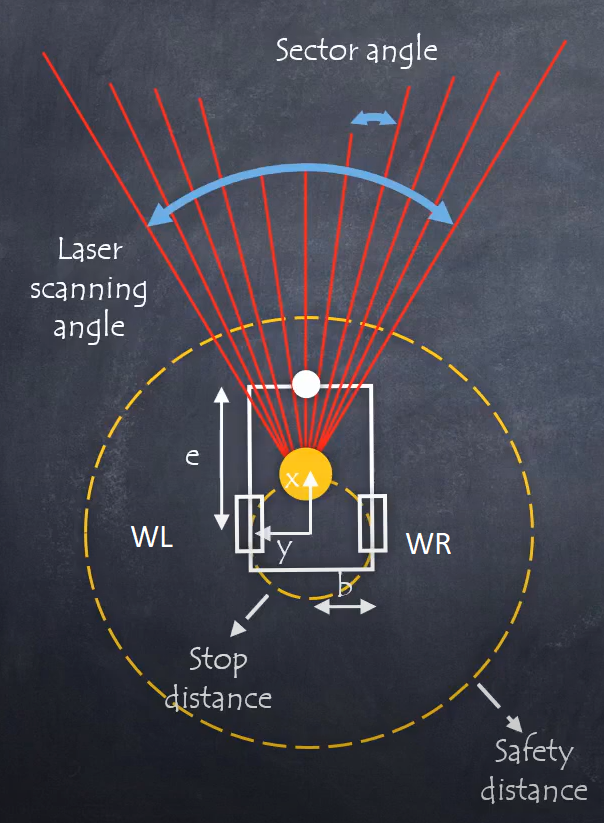
\includegraphics[width= 0.6\textwidth]{Figures/robot features.PNG}
  \caption[Robot Features]{Robot Features}
   \label{fig:Robot Features} \cite{PF}
\end{figure}

\noindent The features are b (distance from one wheel to the robot center line), e (off-kinematic control point), wheel radius, stop distance, safety distance and the amounts are: \\
\begin{align*}
\text{wheel\_radius} &= \frac{0.195}{2} \\
b &= 0.1655 \\
\text{stop\_distance} &= 0.2 \\
\text{safety\_distance} &= 0.55 \\
e &= 0.3\\
\text{scan\_angle} &= \text{math.rad(sim.getUserParameter(hokuyo,'scanAngle'))} \\
\text{cell\_size} &= 0.1 \\
\text{window\_size} &= 2 \times \text{sim.getUserParameter(hokuyo,'maxScanDistance')} \\
\text{sector\_angle} &= \text{math.rad(5)} \\
\text{wide\_sector\_width} &= 5 \\
\tau_{\text{low}} &= 500 \\
\tau_{\text{high}} &= 2000 \\
\text{target\_weight} &= 3 \\
\text{previous\_weight} &= 2 \\
\text{current\_weight} &= 1
\end{align*}
\noindent After making polar histogram, robot uses from two threshold to decide if a sector was occupied or not. If bars in polar histogram are higher than a high threshold then they concluded as occupied means 1  and if bars are lower than a low threshold so they are free mean zero and otherwise the bars in between use as previous iteration value. Then based on the minimum turning radius and kinematic constrains robot decide to mask parts of histogram. After masking parts of binary histogram wide and narrow valleys remains for robot to follow. It is clear that narrow passages can not be more optimised as a route by the robot as the closest path to the goal. But wide valleys can be optimised by 3 items of target weight, previous orientation's weight and robot's orientation weight to minimise the cost function. \\
\noindent To fine-tune the three terms in the cost function formula \eqref{eqn:Cost Function} I tested the variation of target weight (fisrt term) versus time to reach the goal to find the optimised target weight for the robot based on the shortest time. I fixed all parameters except target weight. The results of simulation shown on the Table \ref{table:Variation of Target Weight Versus Time to Reach the Goal}. All the routes passed by robot were the same pattern (here means almost the same distance) in all variations of target weight. The picture of the yellow path is shown from top view in the Figure \ref{fig:Robot Path to Goal}. 

\begin{figure}[H]
  \centering
  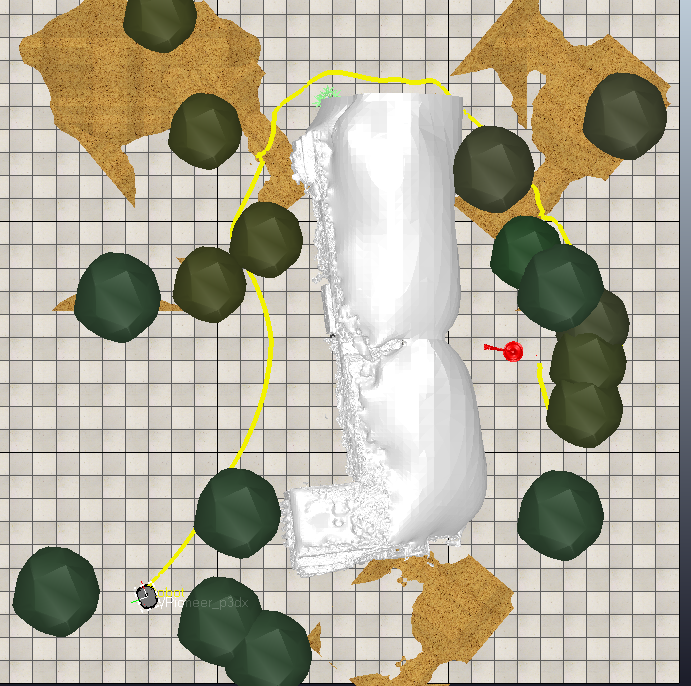
\includegraphics[width= 0.6\textwidth]{Figures/Tw-03.PNG}
  \caption[Robot Path to Goal]{Robot Path to Goal}
   \label{fig:Robot Path to Goal} 
\end{figure}

\begin{table}[ht!]
\centering
    \begin{tabular}{ m{3cm} m{5cm} m{5cm} } 
    \toprule
    \toprule
    \textbf{Target Weight} & \textbf{Reach to Goal or Not} & \textbf{Time to Reach Goal (s)} \\
    \midrule
    1      & 0       &    \\[1.3ex]
    2       & 100    & 77   \\[1.3ex]
    3      & 100     & 76   \\[1.3ex]
    4      & 100     & 91   \\[1.3ex]
    5      & 100    & 91   \\[1.3ex]
    6     & 100     & 104     \\[1.3ex]
    7     & 100     & 75     \\[1.3ex]
    8     & 100     & 75   \\[1.3ex]
    9     & 0       &    \\[1.3ex]
    \bottomrule
    \bottomrule
\end{tabular}
\caption[Variation of Target Weight Versus Time to Reach the Goal]{Table of variation of target weight versus time to reach the goal are based on the same pattern of path. Target weight tested from 1 to 9 numbers, the reach to goal is based on the zero (not reach the goal)and one (reach the goal), the time to reach goal is based on the seconds. }
\label{table:Variation of Target Weight Versus Time to Reach the Goal}
\end{table} 
\noindent With Target Weight (TW) 1 the robot lost in the environment and could not find the path toward goal, seems the low amount of this item cause orientation loss. With TW of 2,the robot passed the obstacles and reached the goal in 77 seconds. In TW of 3,took 76 seconds and in TW of 4 and 5 took 91 seconds for robot to reach the goal, the reason was temporary stuck of robot to the bumps on the terrain due to the structural design of Pionner 3dx robot. In target weight 6, robot had the longest time of stuck after terrain bumps. Finally target weight 7 was the shortest time to reach the goal and the optimised one with 75 seconds. A graph of variation of target weight versus time to reach goal is shown in Figure \ref{fig:Graph of Variation of Target Weight Versus Time to Reach the Goal}. 
\begin{figure}[H]
  \centering
  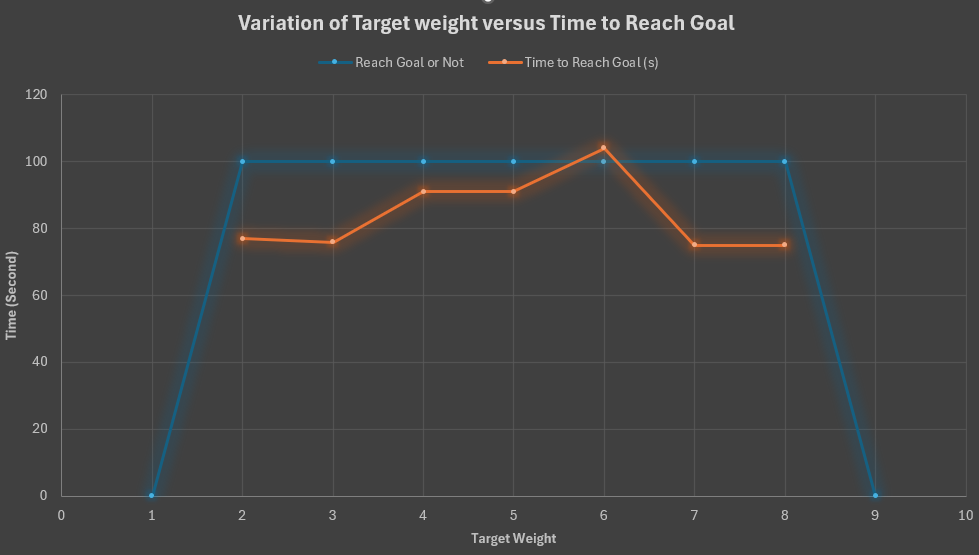
\includegraphics[width= 1.0\textwidth]{Figures/Target vs Time.PNG}
  \caption[Graph of Variation of Target Weight Versus Time to Reach the Goal ]{Graph of Variation of Target Weight Versus Time to Reach the Goal}
   \label{fig:Graph of Variation of Target Weight Versus Time to Reach the Goal} 
\end{figure}


\subsection{Simulation with Vector Field Histogram Plus Method on the deck of a ship with Many obstacles) }
In this environment, robot surrounded by obstacles imported on the deck of a ship to making a complex path for robot to plan the target. In figure \ref{fig:Virtual Robot Simulation on the Deck of a Ship with VFH+ Algorithm} the robot mission on the deck is extinguishing the fire on the shortest time on the other side of the ship to prevent catastrophic consequences of spreading fire. And this simulation proofs the ability of autonomous path planning mobile robots for safer marine operation. 
\begin{figure}[H]
  \centering
  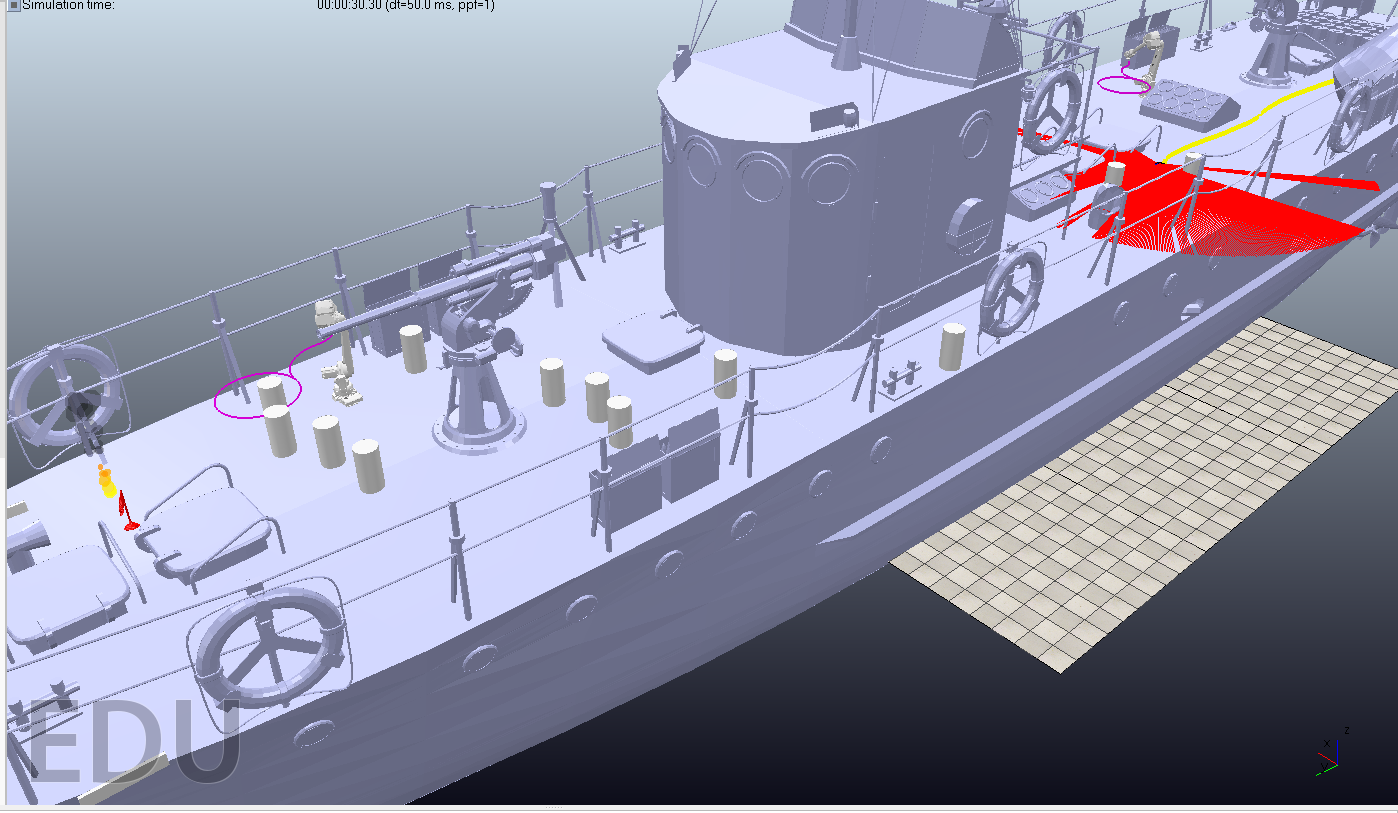
\includegraphics[width= 1.0\textwidth]{Figures/VFH+SHIP.PNG}
  \caption[Virtual Robot Simulation on the Deck of a Ship with VFH+ Algorithm ]{Virtual Robot Simulation on the Deck of a Ship with VFH+ Algorithm}
   \label{fig:Virtual Robot Simulation on the Deck of a Ship with VFH+ Algorithm} 
\end{figure}
\noindent I tested the variation of target weight versus time to reach the fire to find the optimised target weight for the robot based on the shortest time on the deck of a ship. I took constant all parameters except target weight. The results of the simulation shown on the Table \ref{table:Variation of Target Weight Versus Time to Reach the Goal on the Ship}. The picture of the yellow path shown from top view in the Figure \ref{fig:Robot Path with Target Weight of 6} is for target weight of 6 and in Figure \ref{fig:Robot Path with Target Weight of 7} is for target weight of 7. During the testing of different target weight versus time which it is important to mention that the pattern change of robot's path from TW 6 to 7, actually route reduced to reach the goal. And in TW 9, the robot stuck in the turn which is close to industrial robot. 

\begin{figure}[h]
    \centering
    \begin{minipage}{1.0\textwidth}
        \centering
        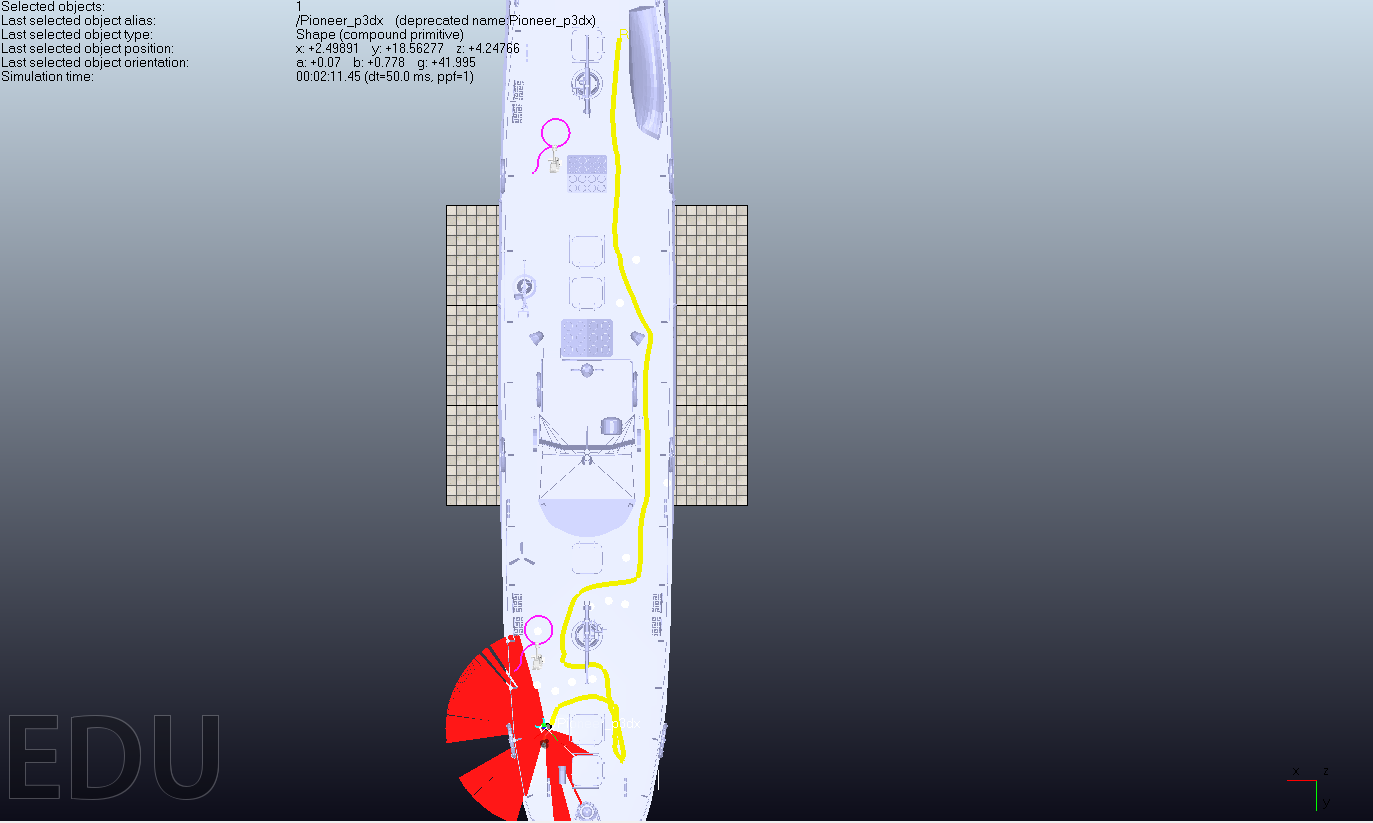
\includegraphics[width=0.9\textwidth]{Figures/TW-6.PNG} % first figure itself
        \caption{Robot Path with Target Weight of 6}
        \label{fig:Robot Path with Target Weight of 6}    
    \end{minipage}\hfill
    \begin{minipage}{1.0\textwidth}
        \centering
        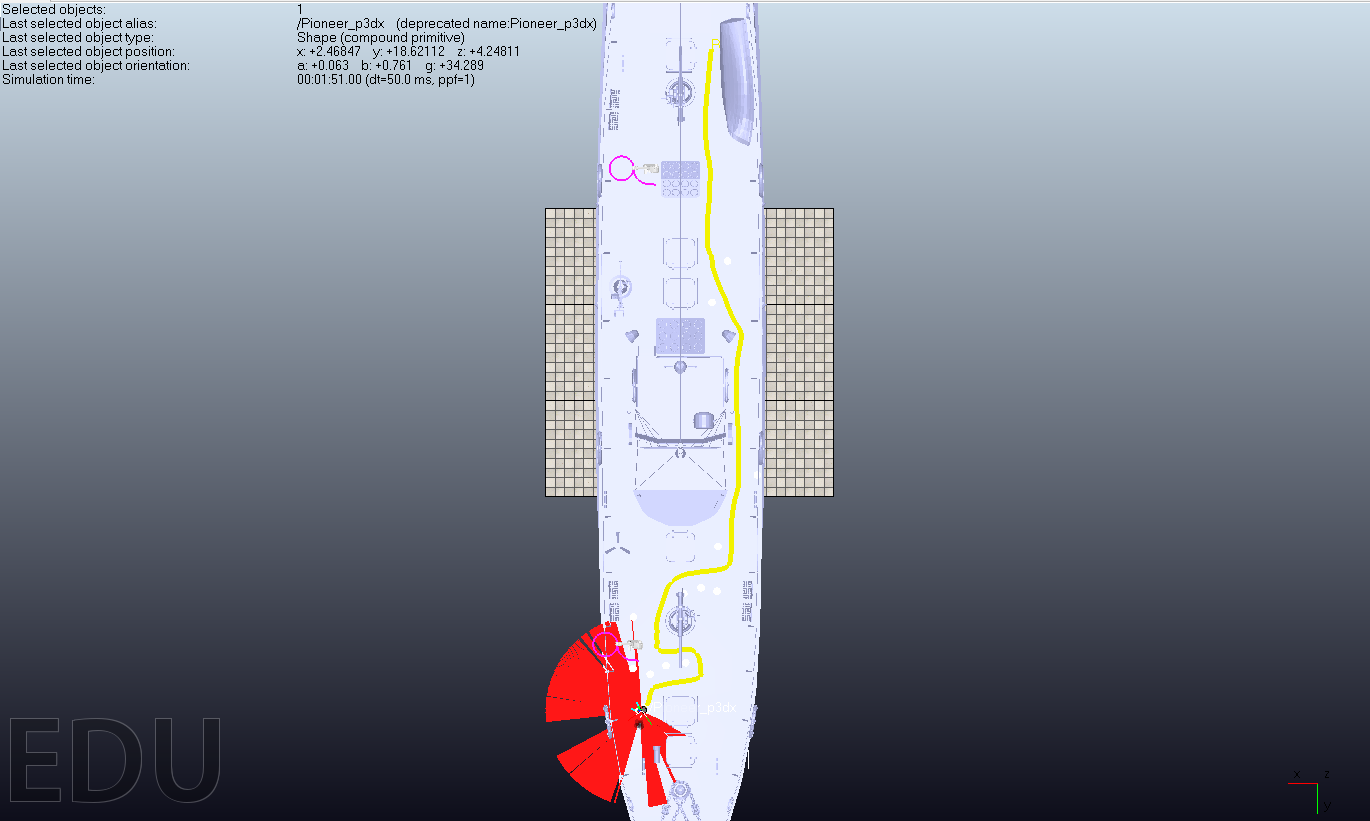
\includegraphics[width=0.9\textwidth]{Figures/TW-7.PNG} 
        \caption{Robot Path with Target Weight of 7} 
        \label{fig:Robot Path with Target Weight of 7}
    \end{minipage}
\end{figure}

\begin{table}[ht!]
\centering
    \begin{tabular}{ m{3cm} m{5cm} m{5cm} } 
    \toprule
    \toprule
    \textbf{Target Weight} & \textbf{Reach to Goal or Not} & \textbf{Time to Reach Goal (s)} \\
    \midrule
    1      & 0       &    \\[1.3ex]
    2       & 0    &    \\[1.3ex]
    3      & 100     & 131   \\[1.3ex]
    4      & 100     & 133   \\[1.3ex]
    5      & 100    & 133   \\[1.3ex]
    6     & 100     & 132     \\[1.3ex]
    7     & 100     & 110     \\[1.3ex]
    8     & 100     & 110   \\[1.3ex]
    9     & 100       & 120   \\[1.3ex]
    10     & 100       & 141   \\[1.3ex]
    11     & 100       & 131   \\[1.3ex]
    12     & 100       & 117   \\[1.3ex]
    13     & 100       & 115   \\[1.3ex]
    14     & 100       & 115   \\[1.3ex]
    15     & 100       &117    \\[1.3ex]
   16     & 100       &117    \\[1.3ex]
    \bottomrule
    \bottomrule
\end{tabular}
\caption[Variation of Target Weight Versus Time to Reach the fire on a Ship's Deck]{Table of variation of target weight versus time to reach the fire. The path of the robot will be shorter by changing the Target Weight from 6 to 7. Target weight tested from 1 to 16 numbers, the reach to goal is based on the zero (not reach the goal)and one (reach the goal), the time to reach goal is based on the seconds. }
\label{table:Variation of Target Weight Versus Time to Reach the Goal on the Ship}
\end{table} 

\noindent In another simulation scenario, I considered the target weight and robot's direction weight constant as 7 and 1 consecutively and changed the Wp (previous direction weight) and checked the goal reach-ability in a specific time and the results is in the table \ref{table:Variation of Previous Direction Weight Versus Time to Reach the Goal on the Ship}. In Wp 7, the robot will be stuck and cannot move anymore. 

\begin{table}[ht!]
\centering
    \begin{tabular}{ m{3cm} m{5cm} m{5cm} } 
    \toprule
    \toprule
    \textbf{Previous Direction Weight} & \textbf{Reach to Goal or Not} & \textbf{Time to Reach Goal (s)} \\
    \midrule
    2      & 100       & 110   \\[1.3ex]
    3      & 100     & 132   \\[1.3ex]
    4      & 100     & 133   \\[1.3ex]
    5      & 100    & 132   \\[1.3ex]
    6     & 100     & 129     \\[1.3ex]
    7     & 0     &      \\[1.3ex]
 
    \bottomrule
    \bottomrule
\end{tabular}
\caption[Variation of Previous Direction Weight Versus Time to Reach the fire on a Ship's Deck]{Table of variation of previous direction weight versus time to reach the fire. Previous direction weight tested from 1 to 7 numbers, the reach to goal is based on the zero (not reach the goal)and one (reach the goal), the time to reach goal is based on the seconds. }
\label{table:Variation of Previous Direction Weight Versus Time to Reach the Goal on the Ship}
\end{table} 
\noindent In another simulation scenario, I considered the target weight and previous direction weight constant as 7 and 2 consecutively and changed the Wc (robot's direction weight) and checked the goal reach-ability in a specific time and the results is in the table \ref{table:Variation of Robot's Direction Weight Versus Time to Reach the Goal on the Ship}. In Wc 4, the robot will stuck and cannot move anymore. 

\begin{table}[ht!]
\centering
    \begin{tabular}{ m{3cm} m{5cm} m{5cm} } 
    \toprule
    \toprule
    \textbf{Robot's Direction Weight} & \textbf{Reach to Goal or Not} & \textbf{Time to Reach Goal (s)} \\
    \midrule
    2      & 100       & 137   \\[1.3ex]
    3      & 100     & 130   \\[1.3ex]
    4      & 0     &    \\[1.3ex]
    
 
    \bottomrule
    \bottomrule
\end{tabular}
\caption[Variation of Robot's Direction Weight Versus Time to Reach the fire on a Ship's Deck]{Table of variation of robot's direction weight versus time to reach the fire. Robot's direction weight tested from 2 to 4 numbers, the reach to goal is based on the zero (not reach the goal)and one (reach the goal), the time to reach goal is based on the seconds. }
\label{table:Variation of Robot's Direction Weight Versus Time to Reach the Goal on the Ship}
\end{table} 
\noindent Based on the cost function formula \eqref{eqn:Cost Function}: 
\begin{equation}
\begin{aligned}
f(c) = W_t \Delta(c,t) + W_p \Delta ( c , p) + W_c \Delta (c)
\end{aligned}
\label{eqn:Cost Function}
\end{equation} 
\\

After several experiments an optimized set of terms for both ship and out-door environment is: 
\begin{align*}
\text{target\_weight} &= 7 \\
\text{previous\_weight} &= 2 \\
\text{current\_weight} &= 1
\end{align*}
\\




\vspace{20cm}

\section{Discussion}

\noindent 1. Simulation in a captured point cloud trigger to a virtual experience of a real environment but if we wanted to use a real robot for simulation can endanger both the robot and the environment, especially in dangerous situations like fire fighting operations.\\

\noindent 2. Virtual environments enable safe testing without the threat of actual injury. Creating and maintaining actual prototypes for real-world testing can be costly. Virtual testing lowers expenses by reducing the requirement for actual prototypes during the early phases of development.\\

\noindent 3. Making design adjustments and testing findings on a real robot can take some time. Virtual environments enable engineers to iterate quickly on design and functionality, hence shortening the development cycle.\\

\noindent 4. It can be difficult to regulate all factors in the real world. Virtual navigation enables exact control over the environment and variables, enabling more detailed and controlled testing situations.\\

\noindent 5. Training operators on actual robots can be dangerous and expensive. Virtual environments offer a safe, controlled setting for training before going on to real-world tasks.  \\

\noindent 6. Collecting data on robot performance and behavior in the real world can be difficult and time intensive. Virtual environments can efficiently capture vast volumes of data, which can then be used to improve robot performance and operational protocols.\\

\noindent 7. Real-world testing necessitates actual presence, which might be restrictive. Virtual testing is accessible from anywhere, allowing teams to interact and train in many locations.\\

\noindent 8. The results showed that Robot stuck several times in potential field algorithms simulation,due to sticking of robot in local minimum, this algorithm was not comparable with VFH+, so I decide to fine tune the VHF+ parameters for different arrangements.   \\

\noindent 9. In the Vector filed histogram plus algorithm in both simulations on the ship and terrain we decided to fine tune the parameters to get an optimized result for our environment. The first term (target weight) drives goal-oriented behavior, while the second and third terms  guide the mobile robot in a specific route. These two terms equip the robot with short-term memory. The third phrase resembles a mechanical memory. The second term allows the robot to commit to a direction before changing its wheel orientation. So the higher target weight means more goal-oriented the robot is. Higher previous robot's direction weight means the more the robot tries to head in the previously set direction. And if the current robot's direction weight  increases, the robot strives for a smooth course with minimal change in direction of travel. 
